%%%%%%%%%%%%%%%%%%%%%%%%%%%%%%%%%%%%%%%%%%%%%%%%%%%%%%%%%%%%%%%%%%%%%%%%%%%%%%%
%% University of Ulm
%%
%% Faculty of Engineering and Computer Science
%% Institute of Measurement, Control and Microtechnology
%%
%%
%% Template for Student Research Projects, Diploma, Bachelor and Master Thesis
%%
%% by order of Dr.-Ing. Michael Buchholz
%% created by Stephan Grensemann 2010
%%%%%%%%%%%%%%%%%%%%%%%%%%%%%%%%%%%%%%%%%%%%%%%%%%%%%%%%%%%%%%%%%%%%%%%%%%%%%%%

\documentclass[]{mrmthesis}     % <-- [your options (see docu)]
%defaults if no options are used: language=de, Master Thesis, confidential=false,namebehindauthortitle=false,

%new since version 1.6: option "namebehindauthortitle" for author title in front of name,
%   new default is title behind name
%Example:  \documentclass[namebehindauthortitle]{mrmthesis} % for title like "Dipl.-Ing. (FH)"

%new since version v1.6: use of biber instead of bibtex8 to generate biblatex labels (i.e. biblatex backend)
%   please set new option "backendbibtex=true" if bibtex8 is used (not recommended, not longer supported)
%   if biber is not part of your (La)TeX distribution, you can get it from http://biblatex-biber.sourceforge.net/

%new since version 1.4: option "confidential" for theses which should not be published
%Example:  \documentclass[confidential]{mrmthesis}

%2015/05/11 v. 1.9b Uni Ulm - Measurement, Control and Microtechnology
%%%%%%%%%%%%%%%%%%%%%%%%%%%%%%%%%%%%%%%%%%%%%%%%%%%%%%%%%%%%%%%%%%%%%%%%%%%%%%%
%loading extra packages / short list of recommended packages

\usepackage{fixltx2e}                  %fix problems in LaTeX that it "`would be nice"' to correct before next LaTeX release
%\usepackage[ansinew]{inputenc}
%note: AMSmath Package is already loaded by mrmthesis to avoid problems with hyperref

%\usepackage{amssymb}                   %special characters in AMS
%\usepackage{amsfonts}                  %TeX fonts from the American Mathematical Society
%\usepackage{dsfont}                    %Doublestroke Font for set symbols, e.g. real numbers \mathds{R}
%\usepackage{amsbsy}                    %producing bold mathematics symbols where appropriate fonts exist
%\usepackage{mathrsfs}                  %Support use of the Raph Smith�s Formal Script font in mathematics
%\usepackage{mathdots}                  %Commands to produce dots in math that respect font size
%\usepackage{upgreek}                   %provides upright greek letters

%\usepackage{siunitx}                   %International System of Units
\usepackage{textcomp}                  %provide many text symbols in the TS1 encoding

%\usepackage{xspace}                    %provides a single command that looks at what comes after it in the command stream,
                                        %and decides whether to insert a space to replace one "eaten" by the TeX command decoder

%\usepackage{float}                     %improved interface for floating objects
%\usepackage{rotating}                  %rotation tools, including rotated full-page floats

%\usepackage{ltxtable}                  %merged tabularx - longtable package
%\usepackage{booktabs}                  %publication quality tables in LaTeX

%\usepackage{listings}                  %Typeset source code listings using LaTeX
%\lstset{language=html,%
%           frameround=fttt,%
%           breaklines=true,%
%           numbers=left,%
%           numberbychapter=true,%
%           captionpos=b,%
%           basicstyle=\scriptsize}%

%%OLD:
%\usepackage{pstricks}                  %set of macros that allow the inclusion of PostScript drawings directly inside LaTeX code
%\usepackage{auto-pst-pdf}              %Package for using pstricks/PSfrag with PDF(La)TeX, requires PERL!
                           % PLEASE NOTE: to use this package you have to add
                           %  "`--enable-write18"' as compiler argument in the
                           %  LaTeX => PDF output-profile (see description in docu)
%
%IF MODIFICATION OF EPS FILES IS NECESSARY, BETTER USE THE NEW PACKAGE pstool
%\usepackage{pstools}
                           % PLEASE NOTE: to use this package you have to add
                           %  "`--enable-write18"' as compiler argument in the
                           %  LaTeX => PDF output-profile (see description in docu)
%
%THE BEST SOLUTION: USE pgfplots/tikz INSTEAD OF EPS FILES (see also tool "matlab2tikz")
%\usepackage{tikz}                      %language for producing vector graphics from a geometric/algebraic description
%\usepackage{pgfplots}                  %draws high-quality function plots in normal or logarithmic scaling

%\usepackage{epstopdf}                  %convert EPS to 'encapsulated' PDF using GhostScript
                           % PLEASE NOTE: to use this package you have to add
                           %  "`--enable-write18"' as compiler argument in the
                           %  LaTeX => PDF output-profile (see description in docu)

%\usepackage{nomencl}                   %produce lists of symbols as in nomenclature
%\ifthenelse{\boolean{en}}{}{\renewcommand{\nomname}{Nomenklatur}}
%\makenomenclature

%%%%%%%%%%%%%%%%%%%%%%%%%%%%%%%%%%%%%%%%%%%%%%%%%%%%%%%%%%%%%%%%%%%%%%%%%%%%%%%

%!!!
%Regarding the compatibility for different platforms and LATEX distributions, the mrmthesis class requires
% "latin1" (ISO 8859-1) encoding of all files. Especially UNIX user should ensure this encoding using the
% options of your preferred editor.
%!!!

%--------------------------------------------------------------
%% set options for mrmbibstyle:
%% url, ISBN, eprint, DOI: content of respective field is never printed if set to false (default)
%% printlanguage: if set to false (default), the language field is never printed. set to true and use standard
%%      biblatex option clearlang to print language fielf for specific languages (see biblatex manual)
%% yearonly: if set true (default), do not print day or month of a publication even if given
%% titlesentencecase: If set to false (default), all titles are written as given in the bib file. If set to true,
%%      all titles of articels, inproceedings etc. (but not booktitle etc.) are transformed to sentence case,
%%      i.e. only the first letter of the title is capital, all other words start with small letters even if
%%      capital letters in the bib file. Use additional curly braces e.g. for abbreviations which should
%%      remain capital letters (as in original bibtex). The command has no effect on entries where the entry
%%      field "hyphenation" is set to e.g. "ngerman".
\ExecuteBibliographyOptions{eprint=false, url=false, isbn=false, doi=false, yearonly=true, printlanguage=false, titlesentencecase=false}

%\ExecuteBibliographyOptions{firstinits=true} %activate, if all given names shall be abbreviated to initials

%%Use field hyphenation for bib entries to set the language of the bib entry, e.g. for correct hyphenation.
%%Do not mix up with the hyphenation command below!
\ExecuteBibliographyOptions{babel=hyphen} %uses hyphenation for language given in entry's hyphenation field (or global language otherwise)


%% Using new command to add bib file, set options for not printing
\addbibresource{my_mrmthesis.bib} % <- type in your bibfile

%% If the above does not work with older versions of biblatex,
%% try the compatibility mode using the folling command instead:
%\bibliography{my_mrmthesis}      % <- type in your bibfile
%--------------------------------------------------------------

%\hyphenation{}                         %insert hyphenations for unknown words


%Datei f�r eigene Kommandos, z.B.


%Typographie: (ben�tigen Package xspace)
%\newcommand{\dasheisst}{\mbox{d.\,h.}\xspace}
%\newcommand{\unteranderem}{\mbox{u.\,a.}\xspace}
%\newcommand{\zumbeispiel}{\mbox{z.\,B.}\xspace}

%Befehl f�r deutsche Anf�hrungszeichen: (ben�tigt babel mit (n)german)
%\shorthandon{"} %bei Einbindung der Command-Datei vor \begin{document} n�tig
%\newcommand{\gq}[1]{"`#1"'} %doppelte Anf�hrungszeichen, Verwendung \gq{in Anf�hrungszeichen}
%\newcommand{\sgq}[1]{\glq #1\grq{}} %einfache Anf�hrungszeichen, Verwendung \sgq{in Anf�hrungszeichen}
%\shorthandoff{"} %bei Einbindung der Command-Datei vor \begin{document} n�tig


%Mathematisches
%%%%%%%%%%%%%%%
%
%Befehl \vm zur Notation von Vektoren und Matrizen in Fettschrift
%\newcommand{\vm}[1]{\protect\ensuremath\boldsymbol{#1}} %ben�tigt Paket amsbsy
%Befehl \vm zur Notation von Vektoren und Matrizen mit Unterstrich:
%\newcommand{\vm}[1]{\protect\ensuremath\underline{#1}}

%Befehl \trans f�r korrekt gesetztes "T" im Mathemodus f�r "Transponiert
%\newcommand{\trans}{^\text{\rm \textup{T}}} %Verwendung: \vm A\trans
%�hnliche Befehle:
%\newcommand{\inv}{^{-1}} %Inverse
%\newcommand{\pinv}{^{\dag}} %Pseudoinverse
%\newcommand{\opt}{\ensuremath ^\star} %Optimale L�sung

%angepasste Versionen f�r optisch besseren Satz bei einigen Buchstaben (z.B. Y,A):
%\newcommand{\transnah}{^{\!\text{\rm \textup{T}}}}
%\newcommand{\invnah}{^{\!-1}}
%\newcommand{\pinvnah}{^{\!\dag}}
%\newcommand{\optnah}{\ensuremath ^{\!\star}}


%aufrechtes "e" f�r die e-Funktion, als Argument die Potenz:
%\newcommand{\efkt}[1]{\ensuremath {{\rm e}}^{#1}}

%Formeln im Text ohne Zeilenumbruch:
%\newcommand{\teq}[1]{\mbox{$#1$}}

%Befehl f�r PT_n-Glied:
%\newcommand{\PT}[1]{\teq{\text{PT}_{#1}}}

%Einheitsmatrix:
%\newcommand{\eye}[1]{\vm{I}}
%mit Dimension:
%%\newcommand{\eye}[1]{\vm{I}_{\!#1}}

%weitere mathematische Funktionen:
%\DeclareMathOperator{\trace}{spur}
%\DeclareMathOperator{\sign}{sign}
%\DeclareMathOperator{\diag}{diag}


%Normen:
%\newcommand{\frobnorm}[1]{\ensuremath \left\| #1 \right\|_\text{F}}
%\newcommand{\zweinorm}[1]{\ensuremath \left\| #1 \right\|_2}
%\newcommand{\vmnorm}[1]{\ensuremath \left\| #1 \right\|}
                   %insert file with self-defined commands. The file exists and contains many examples.

%%%%%%%%%%%%%%%%%%%%%%%%%%%%%%%%%%%%%%%%%%%%%%%%%%%%%%%%%%%%%%%%%%%%%%%%%%%%%%%
%please fill out the following required information
\title{Segmentierung von Punktwolken mit Neuronalen Netzen}
%\descriptiontitle{title for thesis description page with different line-breaks, if necessary} % Default: \title
%\affirmationtitle{title for affirmation page with different line-breaks, if necessary} % Default: \title
\author[m]{Tarik Enderes} %use optional argument [f] for female label, default is [m] for male
%\authortitle{B.\,Sc.} %default: None, please note: use class option namebehindauthortitle if title should be printed in front of the name
\supervisor[m]{Prof. Dr. rer. nat. Vasileios Belagiannis } %use optional argument [f] for female label, default is [m] for male
\examiner{Prof. Dr. rer. nat. Vasileios Belagiannis }
\coexaminer{Prof. Dr.-Ing. Klaus Dietmayer}
\issuedate{18.07.2019}
\submissiondate{31.10.2019}
%\place{}                       %default: Ulm

%%%%since v. 1.4: Possible re-definition of phrases for "confidential"-option
%%%%please note: Normally, there should be no reason to change these phrases
%%%% and changing can cause unwanted behaviour.
%%%\confidentialMainText{}
%%%\confidentialSubText{}

%%%%%%%%%%%%%%%%%%%%%%%%%%%%%%%%%%%%%%%%%%%%%%%%%%%%%%%%%%%%%%%%%%%%%%%%%%%%%%%
%main text
\begin{document}
% - - - - - - - - - - - - - - -
 \frontmatter
\maketitle
%  \projectdescription{\input{doc/projectdescription}}   % the file "projectdescription.tex" should be provided by your supervisor
  \affirmation

  %\extrafrontchapter{Vorwort}{type in your text here} %or some other optional stuff
  \extrafrontchapter{Danksagung}{Ich m�chte ich bei allen bedanken, die mir geholfen haben, diese Arbeit anzufertigen. Insbesondere bedanke ich mich bei Prof. Dr. Vasileios Belagiannis f�r seine kompetente und geduldige Betreuung, sowie seine Vorschl�ge zur Gestaltung des Projekts. Ein besonderer Dank geht auch an Dipl.-Ing. Uwe Kerner und M. Sc. Nico Engel f�r ihre technische Unterst�tzung.}

  \tableofcontents
  %\listoffigures
  %\listoftables
  %\printnomenclature        %PLEASE NOTE: If you don't change the MakeIndex argument
                             % in the output-profile into
                             % "%bm.nlo" -s nomencl.ist -o "%bm.nls", no output will be produced
% - - - - - - - - - - - - - - -
 \mainmatter                       %import chapters (tip: use one tex-file for each chapter)
   \chapter{Einleitung}
	F�r zahlreiche Entwicklungsthemen der heutigen Zeit, wie beispielsweise autonomes Fahren, ist eine pr�zise Erkennung der Umweltbedingungen unerl�sslich. Kameras und Laserscanner finden f�r diesen Zweck oft Verwendung, was die Verarbeitung von Bildern und Punktwolken zu einem verbreiteten Gegenstand moderner Forschung macht. H�ufig wird zur L�sung dieser komplexen Probleme auf Elemente der Neuroinformatik zur�ckgegriffen. \\
	Je nach Anwendungsfeld ist ein bestimmter Grad an Auswertung der gegebenen Daten erforderlich. Diese Arbeit befasst sich mit der Aufgabe, Bilder und Punktwolken zu segmentieren.
	\section{Segmentierung}
		Segmentierung bezeichnet einen Vorgang, bei dem ein Bild nach bestimmten Homogenit�tskriterien in inhaltlich zusammenh�ngende Regionen eingeteilt wird. Von den verschiedenen Ans�tzen, die das erreichen sollen, befasst sich diese Arbeit mit pixelbasierten Verfahren, bei denen jedem Pixel in einem Bild eine Klasse zugeordnet wird. Man unterscheidet zwischen den in \cite{UPSNet} beschriebenen, semantische Segmentierung, Instanz-Segmentierung und panoptische Segmentierung und der in \cite{DBLP:journals/corr/abs-1904-09172} ausgef�hrten Objekt-Segmentierung. F�r weitere Informationen siehe \cite{gonzalez2008digital}.
		\subsection{Semantische Segmentierung}
			Bei der semantischen Segmentierung soll jeder Pixel eine valide Klasse erhalten. Es wird dabei nicht zwischen unterschiedlichen Instanzen einer Objektklasse unterschieden. Wenn beispielsweise auf einem Bild zwei Fahrzeuge zu sehen sind und bei der Segmentierung die Klasse "`Fahrzeug"' zugeteilt werden soll, erhalten die Pixel beider Fahrzeuge das Label "`Fahrzeug"'. Die Anzahl valider Klassen bleibt somit bei jeden prozessierten Bild gleich.\\ Einige Anwendungsgebiete von semantischer Segmentierung sind autonomes Fahren im Gel�nde \cite{OffRoad}, Zellanalyse in der Biomedizin \cite{journals/corr/RonnebergerFB15} und Auswertung von Satellitenbildern f�r Kartographie \cite{DBLP:journals/corr/abs-1904-03983}.
		\subsection{Instanz-Segmentierung}
			Im Gegensatz zur semantischen Segmentierung werden bei der Instanz-Segmentierung nur z�hlbare Objekte betrachtet und deren Instanzen ber�cksichtigt. �bertragen auf vorheriges Beispiel w�rden die Pixel des einen Fahrzeug ein Label wie "`Fahrzeug1"' und die des anderen analog "`Fahrzeug2"' erhalten.\\
			Instanz-Segmentierung findet beispielsweise Anwendung zur Detektion von Personen in Videodaten f�r Verhaltensanalysen und �berwachung \cite{HumanSegmentation}.
		\subsection{Panoptische Segmentierung}
			Die panoptische Segmentierung stellt eine Kombination der vorherigen Segmentations-Arten dar. Z�hlbare Objekte werden demnach nach dem Prinzip der Instanz-Segmentierung und amorphe nach dem der semantischen Segmentierung segmentiert. Die Ergebnisse beider Verfahren werden anschlie�end kombiniert.
		\subsection{Objekt-Segmentierung}
			Bei der Objekt-Segmentierung soll f�r jeden Pixel eines Bildes entschieden werden, ob er Teil des Vorder- oder des Hintergrundes ist, weshalb sie h�ufig als Vordergrund-Hintergrund-Segmentierung bezeichnet wird. Von Interesse ist dabei nur, wo sich Objekte im Bild befinden, nicht, wie bei den anderen Disziplinen, worum es sich handelt. Oft ist das Ziel dabei die Erkennung von Bewegung in Videodaten.\\
			Objekt-Segmentierung findet Verwendung im Bereich der Video�berwachung \cite{ObjSegmentation}.
		
	\section{Ziele und Anforderunen}
		Ziel der Arbeit ist es, ein System zu entwickel, das mit Hilfe von neuronalen Netzen ein Bild semantisch segmentiert und aufgrund der so entstandene Labels auf Pixelebene eine Punktwolke derselben Szene segmentiert. Der Anwendungsbereich des Systems soll autonomes Fahren sein, weshalb Entwicklung und Experimente mit Datens�tzen f�r diesen durchgef�hrt werden. Konkret soll die Ausgabe des Systems Algorithmen f�r Einf�delvorg�nge an Kreuzungen verbessern. Besondere Wichtigkeit kommt daher der Erkennung von Fahrzeugen, Personen und Stra�en zu. Eine Kernanforderung ist dabei Echtzeitf�higkeit. Optimierung der Laufzeit ist also essentiell. Weiterhin soll das System transportabel, leicht zu verwenden, benutzerfreundlich und ressourcenschonend sein.\\
		Die Entwicklung erfolgt in Python mit CUDA-Unterst�tzung unter Verwendung des von Google entwickelten Framework DeepLab, das zur Zeit der Entstehung dieser Arbeit als State-of-the-Art angesehen wird.\\
   \chapter{Literatur}
	\section{Verwandte Arbeiten}
		\subsection{PointNet}
		\subsection{UPSNet}
   \chapter{Theorie}
	
	\section{DeepLab}
		DeepLab ist ein von Google entwickeltes, 2015  in \cite{DeepLab1} vorgestelltes Modell f�r semantische Segmentierung. Bei der in \cite{DeepLab2} vorgestellten Methode wird ein Deep Convolutional Neural Network (DCNN) zum Erzeugen einer Score Map benutzt, die anschlie�end mit einem Conditional Random Field (CRF) zur endg�ltigen Ausgabe weiterverarbeitet wird. Das Verfahren wird in Abbildung \ref{fig:DeepLabAblauf} grob dargestellt.
		
		\begin{figure}
			\centering
			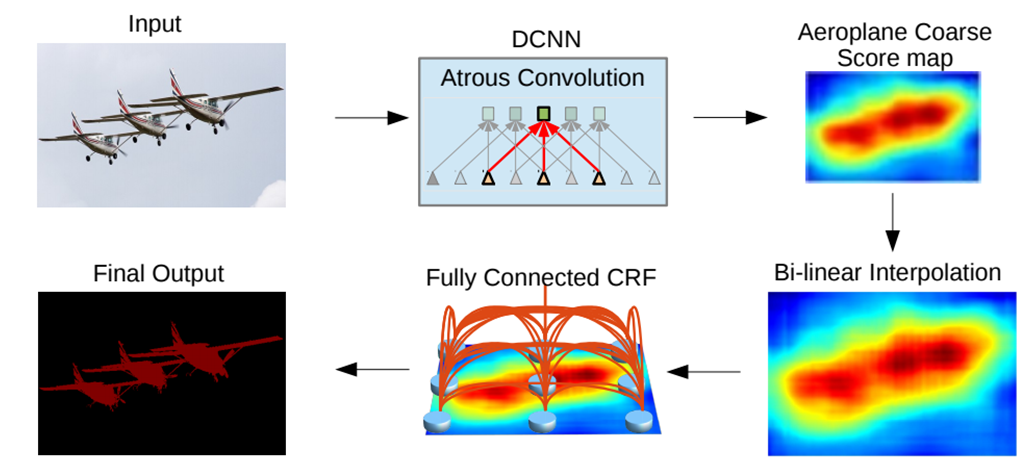
\includegraphics[width = 0.9\linewidth]{img/DeepLabAblauf.png}
			\caption{Grunds�tzliche Funktionsweise von DeepLab}
			\label{fig:DeepLabAblauf}
		\end{figure}  
		\subsection{Deep Convolutional Neural Networks f�r Semantische Segmentierung}
			\subsubsection{Convolutional Neural Networks}
				Wie in \cite{Goodfellow-et-al-2016} beschrieben, handelt es sich bei Convolutional Neural Netzworks (CNNs) um Neuronale Netze, die in mindestens einer Verarbeitungsschicht Faltung an Stelle von Matrixmultiplikation als mathematische Operation durchf�hren. Der Begriff Faltung bezieht sich dabei nicht auf die streng mathematischen Definition. In der Regel wird eine Variation eingesetzt. Verwendet das Netz ausschlie�lich Faltung spricht man von einem Fully Convolution Neural Netzwork. CNNs eignen sich zur Anwendung auf rasterf�rmige Datenstrukturen und werden aufgrund ihrer im Folgenden beschriebenen Eigenschaften h�ufig zur Bildverarbeitung eingesetzt.\\
				Ein Vorteil von Faltung gegen�ber Matrixmultiplikation ist, dass Gr��e der Eingabematrix variabel ist. Im Fall von Bildbearbeitung bedeutet das, dass ein Fully Convolution Neural Netzwork Bilder unabh�ngig von deren Gr��e und Aufl�sung verarbeiten kann. Es ist zu beachten, dass damit nicht Gr��eninvarianz erreicht wird.\\
				Bei der Faltung einer Matrix mit einem Kernel ist jeder Wert des Ergebnisses nur abh�ngig von bestimmten Werten der Eingabematrix, nicht unbedingt von allen, wie bei einer Matrixmultiplikation. F�r semantische Segmentierung bedeutet das, dass der Ausgabewert f�r einen Pixel nur von Pixeln in einem begrenzten Bereich des Eingabebildes, dem Sichtfeld, bestimmt wird. Durch Verkn�pfung mehrerer Faltungsschichten wird dieses Sichtfeld vergr��ert. Au�erdem wird jeder Wert der Eingabematrix auf dieselbe Weise verarbeitet. Damit werden die Ergebnisse der Faltungsschichten in einem Netzwerk Equivariant gegen�ber Translation. Das bedeutet, wenn die Eingabe verschoben ist, tritt die gleichen Verschiebung in der Ausgabe auf. Die Gr��e des Faltungskernels kann theoretisch frei gew�hlt werden und ist im Fall von Bildverarbeitung vernachl�ssigbar klein verglichen mit den Eingabedaten, was CNNs deutlich effizienter im Bezug auf Laufzeit und besonders Speicherbedarf macht.\\
				�blicherweise wird in CNNs eine Pooling genannte Operation eingesetzt. Beim Pooling wird aus einer Matrix eine andere, meistens kleinere erstellt, die eine Zusammenfassung der Originalmatrix darstellt. Es gibt verschiedene Arten von Pooling. H�ufig verwendet wird s.g. Max-Pooling, bei dem jeder Eintrag der Ausgabematrix das Maximum eines rechteckigen Bereichs der Eingabematrix ist. Durch Pooling soll das Netz Resistenter gegen�ber kleinen �nderungen der Eingabedaten werden und die Gr��e f�r weitere Verarbeitungsschichten verringert werden um die Laufzeit zu verbessern. Typischerweise folgt eine Pooling-Schicht auf eine oder mehrere Faltungsschichten. 
			\subsubsection{Anpassungen f�r Semantische Segmentierung}
				Klassische DCNNs haben Eigenschaften, die sie f�r die Verwendung zur Bildsegmentierung nicht ideal machen. 
				\begin{itemize}
					\item Der Einsatz von Downsampling f�hrt zu verringerter Aufl�sung, die bei Klassifizierungsaufgaben nicht ins Gewicht f�llt, f�r die Segmentierung aber essentiell ist. 
					\item Neuronale Netze sind in der Regel gut geeignet, um Objekte unterschiedlicher Gr��e zu erkennen, wenn solche in der Lernphase pr�sentiert werden. Die Eigenschaften der Faltung, insbesondere dem begrenzten Sichtbereich beim Berechnen eines einzelnen Pixels ist allerdings f�r diese Problematik ung�nstig.
					\item Der wiederholte Einsatz von Convolutional Layers f�hren zu einem Verlust an Ortsinformation. Infolgedessen produzieren DCNNs bei Segmentierungsaufgaben verschwommene, oft verrauschte Ergebnisse ohne klare Kanten.
				\end{itemize}
			
			Um diese Probleme zu l�sen erh�lt das von DeepLab verwendete DCNN einige Anpassungen. Zun�chst werden alle Fully Connected Layers durch Convolutional Layers ersetzt, um ein Fully Convolutional Network zu bilden. 
			Noch dazu wird anstatt von Pooling Layers in den unteren Schichten Atrous Convolution eingesetzt, womit die Aufl�sung der Ausgabe erh�ht wird. In den h�heren Schichten werden auch hier Pooling Layers eingesetzt, um Speicherbedarf und Rechenzeit zu verbessern. 
			Um die Gr��eninvarianz zu verbessern wird bei den unteren Schichten Atrous Spatial Pyramid Pooling verwendet.
			
		\subsection{Atrous Convolution}
			Atrous Convolution, auch Dilated Convolution genannt, beschreibt eine Technik bei der eine Matrix mit einem sp�rlich best�ckten Kernel gefaltet wird, wie in Abbildung \ref{fig:AtrousConv} illustriert.
			
				\begin{figure}
					\centering
					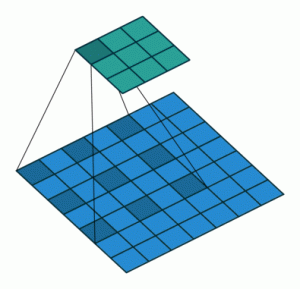
\includegraphics[]{img/AtrousConv.png}
					\caption{Prinzip von Atrous Convolution}
					\label{fig:AtrousConv}
				\end{figure} 
			Die Abst�nde der zu ber�cksichtigenden Werte in der Matrix wird dabei durch die s.g. Dilation Rate bzw. Erweiterungsrate (kurz Rate) festgelegt. Das Tats�chliche Sichtfeld des Filters wird also festgelegt durch die Gr��e des Kernels und die Rate bestimmt.\\ ein Filter mit einem Kernel der Gr��e 3x3 und einer Rate von 2, was dem Einf�gen einer leeren Zeilen und Spalte zwischen den Werten entspricht, hat demnach ein Sichtfeld der Gr��e 5x5.
			Dadurch wird das effektive Sichtfeld des Filters erh�ht und es kann eine h�here Aufl�sung bei gleichen Rechenaufwand erreicht werden. Die Vorteile der Verwendung von Atrous Convolution f�r Bildsegmentierung sind in Abbildung \ref{fig:AtrousConvRes} dargestellt.
				\begin{figure}
					\centering
					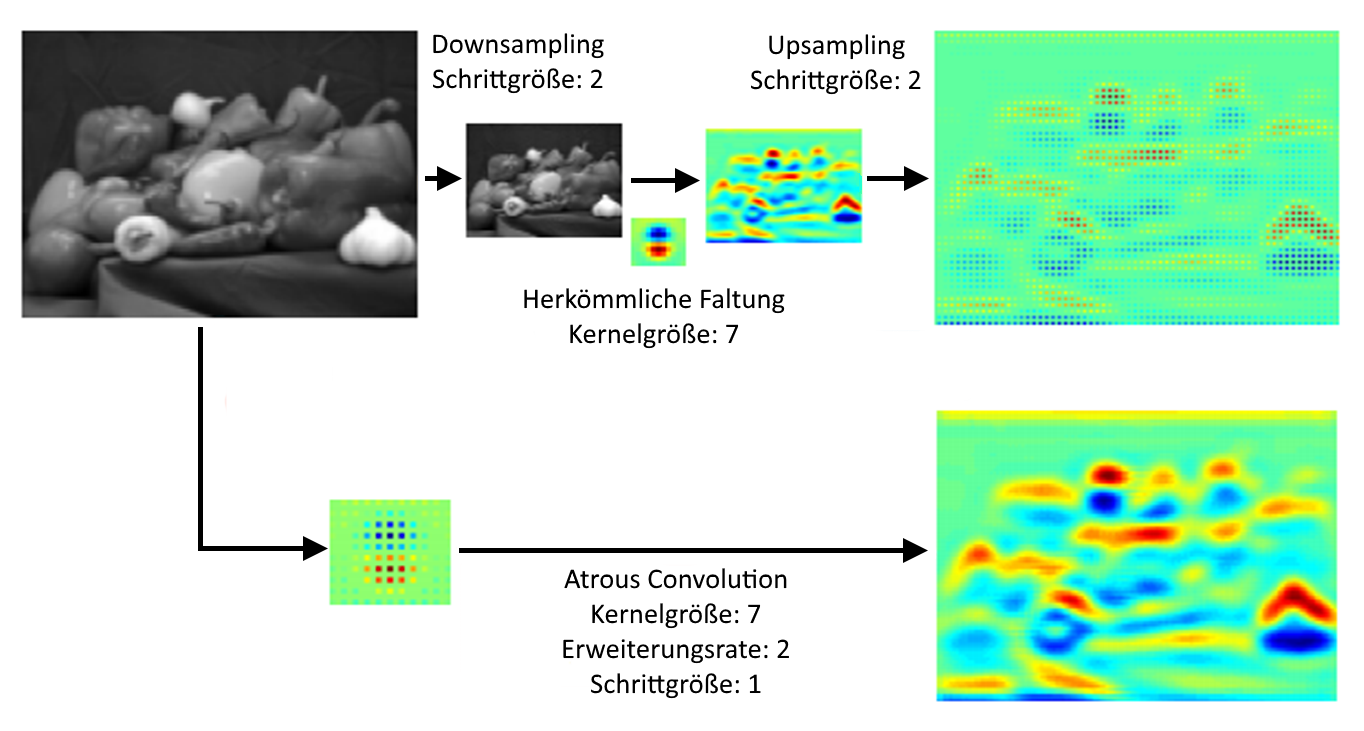
\includegraphics[width = 0.9\linewidth]{img/AtrousConvRes.png}
					\caption{Beispielhaft dargestellte Vorteile von Atrous Convolution}
					\label{fig:AtrousConvRes}
				\end{figure} 
		
		\subsection{Atrous Spatial Pyramid Pooling}
			Beim Atrous Spatial Pyramid Pooling werden mehrere parallele Convolutional Layers, die Atrous Convolutional Layers mit unterschiedlicher Rate verwenden, in das DCNN eingebaut. Das Prinzip ist in Abbildung \ref{fig:PyramPooling} dargestellt.\\
			Durch dieses Vorgehen soll Gr��eninvarianz erreicht werden.
			
				\begin{figure}
					\centering
					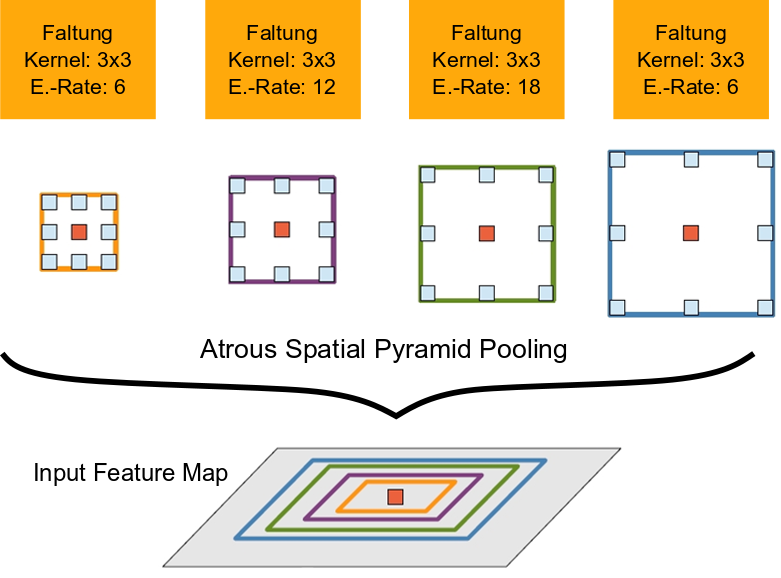
\includegraphics[width = 0.9\linewidth]{img/PyramPooling.png}
					\caption{Beispielhaft dargestellte Vorteile von Atrous Convolution}
					\label{fig:PyramPooling}
				\end{figure} 
		\subsection{Fully-Connected Conditional Random Fields}
		\subsection{Residual Networks}
			Ein Residual Neural Networks (ResNet) ist ein neuronales Netz, das das in \cite{DBLP:journals/corr/HeZRS15} vorgestellte Residual Learning implementiert. Dabei werden, wie in \ref{fig:ResNet} dargestellt, "`Abk�rzungen"' in das Netz eingebaut, �ber die die Ausgabewerte einer Schicht eine oder mehrere nachfolgende Schichten �berspringen und eine tiefere Schicht unver�ndert erreichen und mit den Ergebnissen der �bersprungenen Schichten kombiniert werden.\\
			\begin{figure}
				\centering
				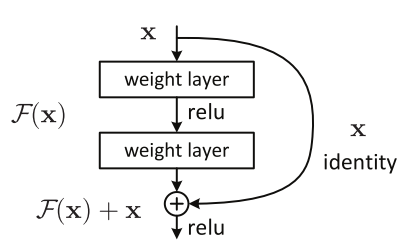
\includegraphics[]{img/ResNet.png}
				\caption{Prinzip von Residual Learning}
				\label{fig:ResNet}
			\end{figure} Mit ResNets wird ein Problem von Deep Neural Networks gel�st, bei dem der Trainingsfehler durch Hinzuf�gen zus�tzlicher Verarbeitungsschichten vergr��ert wird.
			
	\section{Kamerakalibrierung}
		
   \chapter{Arbeitsmethodik und Entwicklung}
	\section{Algorithmus}
		\label{sec:algo}
		Es gibt mehrere Ans�tze zum Segmentieren von Punktwolken mit Neuronalen Netzen, die unterschiedliche Leistungen bez�glich Laufzeit und Qualit�t erzielen. In dieser Arbeit wird ein m�glichst einfacher und zeiteffizienter Algorithmus angewandt. Dabei wird, wie in Abbildung \ref{fig:Verfahren} dargestellt, zuerst ein Eingabebild mit Hilfe Neuronaler Netze semantisch segmentiert. Dazu wird an dieser Stelle DeepLabV3+ \cite{DBLP:journals/corr/abs-1802-02611} benutzt, da es mit seinen Ergebnissen auf popul�ren Datens�tzen (79.7\% auf Pascal VOC 2012 \cite{Everingham10} und 70.4\% auf Cityscapes \cite{Cityscapes} in mIOU-Metrik) laut \cite{DeepLab2}, als State-of-the-Art angesehen wird und gleichzeitig eine gro�e F�lle an Informationen und �ffentlichen Implementierungen zur Verf�gung stehen. \\
		Die durch die Segmentierung ermittelten Labels werden anschlie�end auf eine Punktwolke projiziert, die dieselbe Szene wie das segmentierte Bild darstellt. Dazu werden ein Bild und eine Punktwolke der zu segmentierenden Szene, sowie eine Projektionsmatrix ben�tigt. die verwendete Kamera muss also kalibriert sein. Offensichtlich ist es damit nur m�glich, den Bereich der Punktwolke zu segmentieren, der im Bild zu sehen ist. Au�erdem werden auf diese Weise keine in der Punktwolke vorhandenen Tiefen-Information ausgenutzt. Stattdessen k�nnen Farb-Informationen ber�cksichtigt werden.
		\begin{figure}[h]
			\centering
			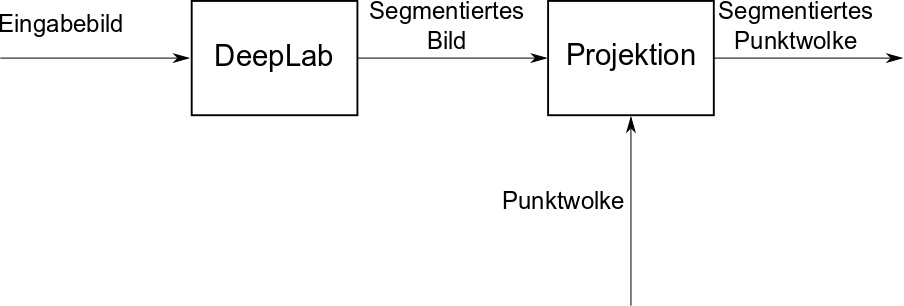
\includegraphics[width = 1\linewidth]{img/Verfahren.png}
			\caption{Schematische Arbeitsweise des Systems. Ein Eingabebild wird zun�chst mit DeepLab segmentiert. Die so entstandenen Labels werden unter Verwendung einer Projektionsmatrix auf eine zum Eingabebild geh�rende Punktwolke projiziert.}
			\label{fig:Verfahren}
		\end{figure}
	\section{DeepLab} \label{sec:dl}
		DeepLab ist ein von Google entwickeltes, 2015  in \cite{DeepLab1} vorgestelltes Modell f�r semantische Segmentierung. Bei der in \cite{DeepLab2} vorgestellten Methode wird ein Deep Convolutional Neural Network (DCNN) zum Erzeugen einer Score Map benutzt, die anschlie�end mit einem Conditional Random Field (CRF) zur endg�ltigen Ausgabe weiterverarbeitet wird. Das Verfahren wird in Abbildung \ref{fig:DeepLabAblauf} grob dargestellt.
		
		\begin{figure}[h]
			\centering
			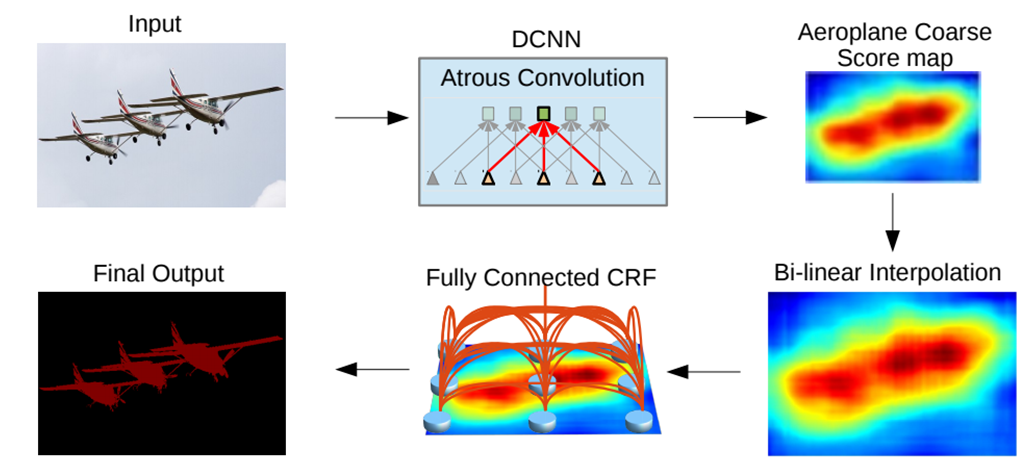
\includegraphics[width = 0.9\linewidth]{img/DeepLabAblauf.png}
			\caption{Arbeitsfluss von DeepLab nach \cite{DeepLab2}. Das Eingabebild wird von einem DCNN segmentiert. Das Ergebnis wird durch Bilineare Interpolation auf die Gr��e der Eingabe vergr��ert und in einem Fully Connected CRF raffiniert.}
			\label{fig:DeepLabAblauf}
		\end{figure}  
		
		\subsection{Anpassungen f�r Semantische Segmentierung}
		Klassische DCNNs haben Eigenschaften, die sie f�r die Verwendung zur Bildsegmentierung nicht ideal machen. 
		\begin{itemize}
			\item Der Einsatz von Downsampling f�hrt zu verringerter Aufl�sung, die bei Klassifizierungsaufgaben nicht ins Gewicht f�llt, f�r die Segmentierung aber essentiell ist. 
			\item Neuronale Netze sind in der Regel gut geeignet, um Objekte unterschiedlicher Gr��e zu erkennen, wenn solche in der Lernphase pr�sentiert werden. Die Eigenschaften der Faltung, insbesondere dem begrenzten Sichtbereich beim Berechnen eines einzelnen Pixels ist allerdings f�r diese Problematik ung�nstig.
			\item Der wiederholte Einsatz von Convolutional Layers f�hrt zu einem Verlust an Ortsinformation. Infolgedessen produzieren DCNNs bei Segmentierungs-Aufgaben verschwommene, oft verrauschte Ergebnisse ohne klare Kanten.
		\end{itemize}
		
		Um diese Probleme zu l�sen, erh�lt das von DeepLab verwendete DCNN einige Anpassungen. Zun�chst werden alle Fully Connected Layers durch Convolutional Layers ersetzt, um ein Fully Convolutional Network zu bilden. 
		Noch dazu wird anstatt von Pooling Layers in den unteren Schichten Atrous Convolution eingesetzt, womit die Aufl�sung der Ausgabe erh�ht wird. In den h�heren Schichten werden auch hier Pooling Layers eingesetzt, um Speicherbedarf und Rechenzeit zu verbessern. 
		Um Gr��eninvarianz zu erreichen wird bei den unteren Schichten Atrous Spatial Pyramid Pooling verwendet und um die Ergebnisse, vor allem an den Kanten von Objekten zu verbessern und Rauschen zu reduzieren, wird die Ausgabe des DCNN mit einem Fully Connected CRF weiterverarbeitet.


	\section{Anwendung von DeepLab}
		Als Basis f�r die Anwendung von DeepLab dient eine �ffentlich zug�ngliche Implementierung in Python mit dem Pytorch-Framework. \\
		Das Projekt implementiert die zwei Netzwerke Xception65 und MobileNetV2. Es wird die M�glichkeit angeboten, vor-trainierte Encoder zu verwenden, die in dieser Arbeit aber nicht genutzt wird, da derzeit Kompatibilit�tsprobleme mit den bereitgestellten vor-trainierten MobileNetV2-Models auftreten. Neben den bereits beschriebenen Technologien werden die klassischeren Konzepte der Neuroinformatik Dropout, L2-Regularisierung und Momentum verwendet, die in \cite{Goodfellow-et-al-2016} nachgeschlagen werden k�nnen.\\
		Bez�glich der Entwicklung ist das erste Ziel die Verwendung dieses Projekts mit einem vor-trainierten Model zur Evaluierung frei gew�hlter Bilder. Ein Model bezeichnet im Rahmen dieser Arbeit eine Datei, in der vom Netz gelernte Parameter gespeichert sind und bei Bedarf geladen werden k�nnen. Die urspr�ngliche Implementierung erwartet Test- und Trainingsdaten im Format von entweder Cityscapes oder Pascal. Der erste Schritt ist folglich die Erstellung eines Python-Skripts zur Evaluierung beliebiger Bilder. Dieses Skript soll Ausgaben im PNG-Format erzeugen, die das Originalbild, die Auswertung des Netzes, eine Legende, ein RGP-Histogramm und die erforderte Rechendauer zeigen. Zur Erzeugung der Plots wird das Modul Matplotlib verwendet. F�r den Fall, dass die Eingabebilder einen schwarzen Rand aufweisen, wird dieser Rand auf die segmentierten Bilder �bertragen, wozu das Bildverarbeitungs-Framework OpenCV verwendet wird. Die Legende wird automatisch erstellt und richtet sich nach der Klasse mit dem h�chsten Label, die in dem Eingabebild erkannt wurde. Sie zeigt au�erdem den IoU-Wert jeder Klasse. Das RGB-Histogramm wird mit einer Funktion von OpenCV automatisch erstellt. Ein Beispiel ist in Abbildung \ref{fig:BspPr} dargestellt.\\
		\begin{figure}[h!]
			\centering
			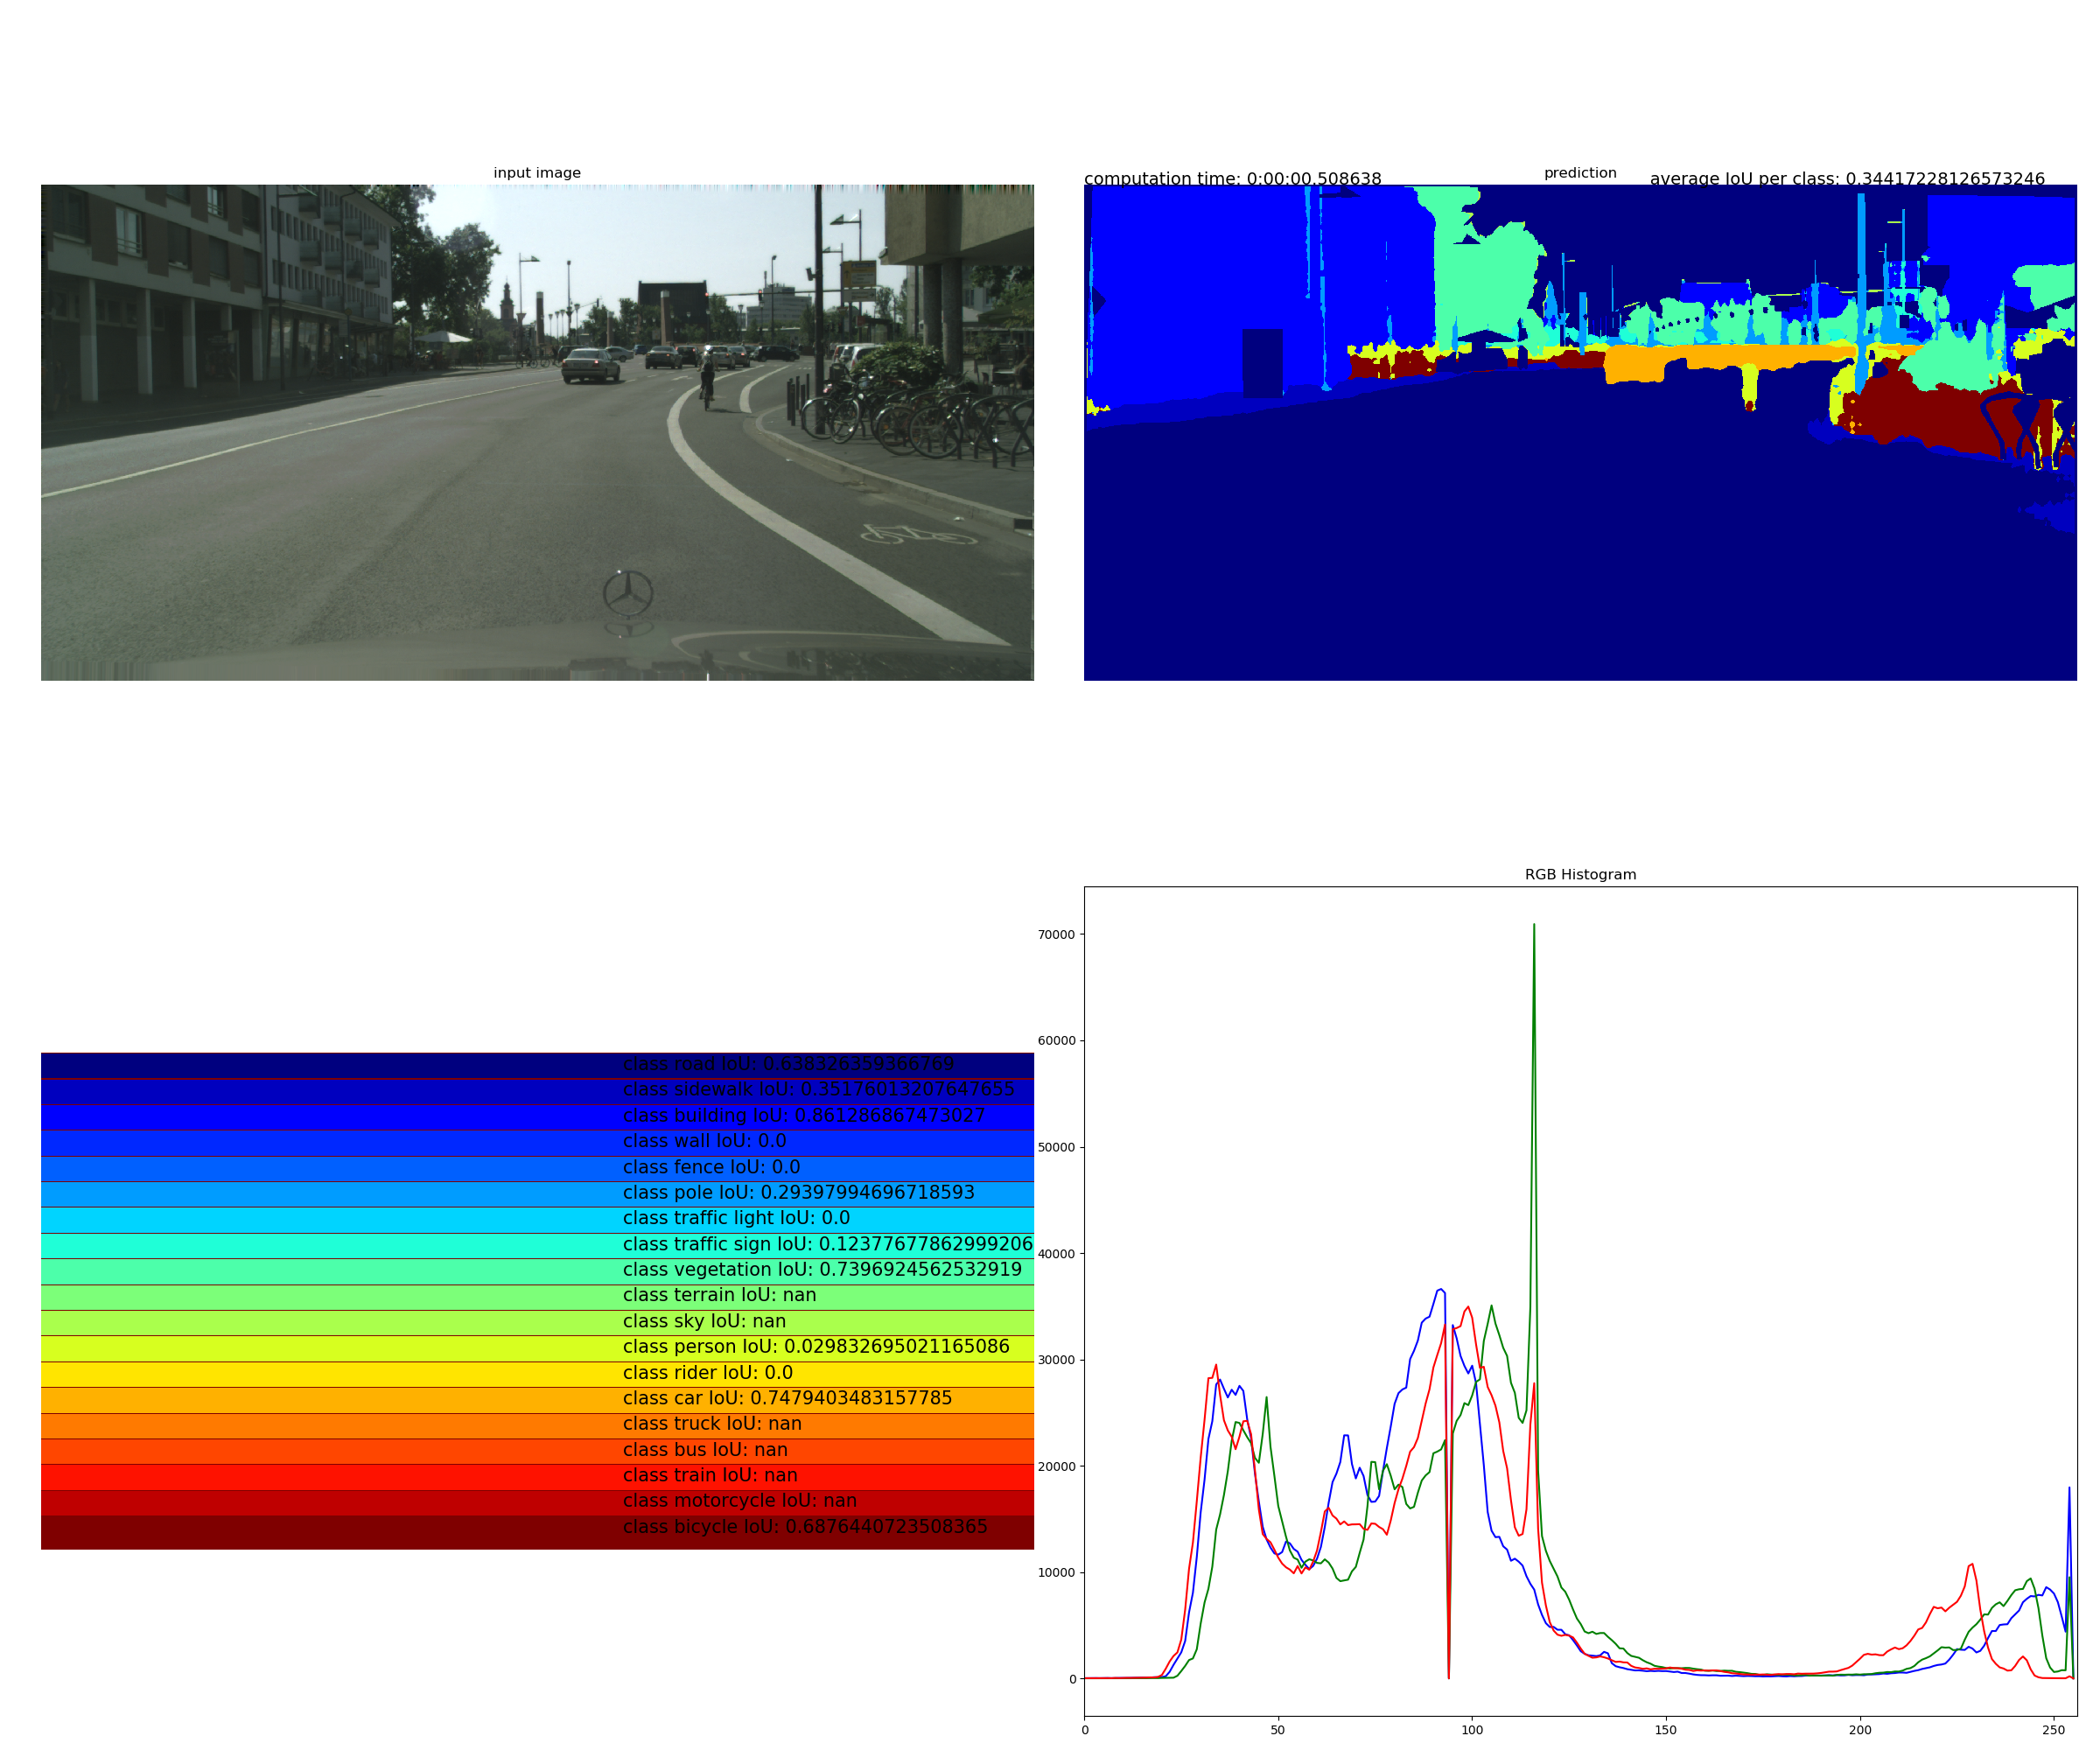
\includegraphics[width=15cm]{img/BeispielErgebnis.png}
			\caption{Beispiel f�r die Ausgabe des Evaluierungs-Skripts. Zu sehen ist das Eingabebild (oben links), das segmentierte Bild (oben rechts), eine Legende, die den IoU f�r jede Klasse enth�lt (unten links) und ein RGB-Farbhistogramm (unten rechts). Die Rechenzeit des Netzes und der durchschnittliche IoU werden �ber dem segmentierten Bild angezeigt.}
			\label{fig:BspPr}
		\end{figure}
		In einem n�chsten Schritt soll die M�glichkeit geschaffen werden, ein eigenes Model mit eigenen Trainingsdaten zu trainieren. Das bereits vorhandene Trainings-Skript kann dazu verwendet werden. Die Verwendung von Nebenl�ufigkeit beim Laden der Trainingsdaten f�hrt allerdings unter Windows dazu, dass das Training nach einer Epoche abgebrochen wird. Auch hier wird erwartet, dass die Daten im Format von Cityscapes oder Pascal sind. Da hier vor allem der Cityscapes-Datensatz zum Trainieren verwendet wird und dieser einfach zu erweitern ist, wird das als sinnvoll eingesch�tzt und beibehalten. Zum Beginnen eines Trainings muss eine Konfigurationsdatei im YAML-Format �bergeben werden. Darin k�nnen folgende Trainingsparameter festgelegt werden:
		\begin{itemize}
			\item Encoder-Type
			\item Decoder-Typ
			\item Format des Datensatzes
			\item Zielgr��e der Trainingsbilder
			\item Anzahl Trainingsepochen
			\item Batch-Gr��e
			\item Verwendung von FP16
			\item Fehler-Typ
			\item zu ignorierender Index (255 in Cityscapes)
			\item Optimierer
			\item Grundlernrate
		\end{itemize}
		Au�erdem kann der Pfad zu einem vor-trainierten Model angegeben werden und bestimmt werden, ob ein bereits existierendes Model weiter trainiert werden soll, was zum Nach-Training benutzt werden kann. \\
		Als letztes muss noch ein Skript erstellt werden, das ein Model auf dem Cityscapes-Datensatz testet und in IoU-Metrik bewertet. Eine Funktion zur Berechnung des IoU ist bereits vorhanden, muss aber noch in einer f�r diese Arbeit sinnvolle Weise aufgerufen werden. Das dazu geschriebene Skript erwartet Evaluierungsdaten im Cityscapes-Format, da die Experimente auf diesem Datensatz durchgef�hrt werden. Es wertet alle Bilder dieses Datensatzes mit dem zu testenden Model aus und berechnet den durchschnittlichen IoU f�r jede von dem Netz erkennbare Klassen, sowie die durchschnittliche Rechendauer pro Eingabebild. Zu beachten ist dabei, dass NaN-Werte bei der Berechnung speziell behandelt werden m�ssen.\\
		Zus�tzlich soll noch die M�glichkeit geschaffen werden, eigene Daten zu annotieren. Dazu wird der von der University of Oxford bereitgestellte VGG Image Annotator (VIA) genutzt. Dieser bietet die M�glichkeit, Polygone in ein Bild einzutragen und diese als CSS-Dateien zu exportieren. Ein Python-Skript, das OpenCV verwendet verarbeitet diese Daten dann zu Cityscapes-konformen PNG-Dateien, die zum Training oder zur Validierung verwendet werden k�nnen. Im Rahmen dieser Arbeit wird das allerdings nicht eingesetzt.
	\section{Backbones}
		Wie bereits erw�hnt, wird der Begriff Backbone hier als Synonym f�r Feature Extractor verwendet und bezeichnet ein Netz, das ein Bild als Eingabe erh�lt und eine Feature Map erzeugt. Die hier verwendete Implementierung von DeepLab umfasst zwei Backbones: Xception65 und MobileNetV2.
		\subsection{Xecption}
			Das in \cite{Xception} pr�sentierte Xception-Netzwerk ist ein einfaches aber leistungsf�higes DCNN, das auf der Idee von Depthwise Separable Convolution basiert. Es wird also angenommen, dass Korrelationen, die mehrere Kan�le umfassen von r�umlichen Korrelationen entkoppelt werden k�nnen. Die einzelnen Module des Netzes verarbeiten zun�chst alle Kan�le separat und f�hren dann eine einfache Faltung �ber alle Dimensionen durch. Dadurch werden Laufzeit- und Speichereffizienz verbessert. Das Prinzip ist in Abbildung \ref{fig:SepConv} dargestellt.\\
			\begin{figure}[h!]
				\centering
				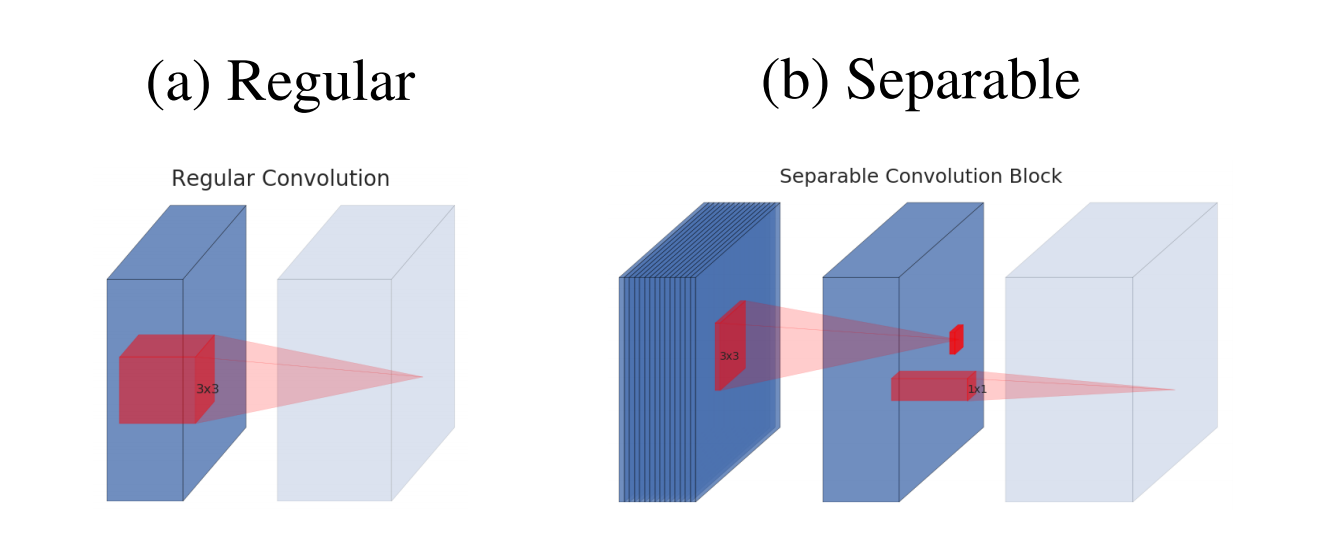
\includegraphics[width=15cm]{img/SeparableConvolution.png}
				\caption{Schematische Darstellung des Prinzips von Depthwise Separable Convolution zur Tensorverarbeitung nach \cite{MobileNetV2}. Statt einer Faltung mit einem 3x3-Kernel �ber alle Dimensionen, wird f�r jede Dimension eine Faltung mit einem 3x3-Kernel durchgef�hrt, gefolgt von einer Faltung mit einem 1x1-Kernel �ber alle Dimensionen.}
				\label{fig:SepConv}
			\end{figure}
			Das vorgestellte Netz hat insgesamt 36 Faltungsschichten, die in 14 Module gegliedert sind, die als ResNet miteinander verbunden sind. In jeder Schicht werden nach dem oben erkl�rten Prinzip mehrere Faltungen mit 3x3 Filtern parallel auf allen Kan�len durchgef�hrt. Der so entstandene Tensor wird anschlie�end mit einem 1x1 Filter gefaltet, der alle Dimensionen umfasst.
		\subsection{MobileNetV2}
			Bei MobileNetV2 \cite{MobileNetV2} handelt es sich um ein leichtgewichtiges DCNN f�r die Implementierung auf mobilen Ger�ten. Da Laufzeit und Ressourcenlastigkeit f�r das Ziel dieser Arbeit von kritischer Bedeutung sind, wird hier vorrangig mit diesem Backbone gearbeitet. Wie Xception verwendet es das Prinzip von Depthwise Separable Convolution und Residual Connections. F�r den Entwurf des Netzes wird zus�tzlich die Annahme gemacht, dass die entscheidenden Eigenschaften eines Eingabetensors in einem Subraum mit weniger Dimensionen zusammengefasst werden k�nnen.\\
			Begr�ndet auf diesen Konzepten ist das grunds�tzliche Architekturelement von MobileNet der so genannte "`Bottleneck Residual Block"'. Ein- und Ausgabetensoren dieser Verarbeitungsschichten haben eine niedrigere Dimension als Tensoren dazwischen. Innerhalb des Blocks wird zuerst der Eingabetensor zu einem mit mehr Dimensionen erweitert. Der so entstandene Tensor wird dann nach dem Prinzip von Depthwise Separable Convolution zuerst Kanalweise, dann Kanal�bergreifend mittels Faltungsoperationen und ReLU6 weiterverarbeitet, wobei die Dimension wieder reduziert wird. Das Ergebnis davon wird nach dem ResNet-Prinzip mit dem Eingabetensor verrechnet. Der Vorteil dieses Verfahrens liegt in einem geringeren Speicherbedarf. Insgesamt besteht das Netz aus einem Convolutional Layer mit 32 Filtern am Anfang, gefolgt von 19 Residual Bottleneck Layer und einigen weiteren Schichten am Ende, die von der zu erf�llenden Aufgabe abh�ngig sind.\\
			
	\section{Segmentierung von Punktwolken}
		Wie in Abschnitt \ref{sec:cam} beschrieben, ist es durch Kenntnis einer Projektionsmatrix m�glich zu berechnen, wo ein Punkt im dreidimensionalen Raum auf einem aufgenommenen Bild erscheint. Ist eine solche Matrix f�r die jeweilige Kamera bekannt, wird diese als kalibriert bezeichnet. \\Zur Projektion der auf dem Bild erkannten Klassen auf die Punktwolke iteriert ein Algorithmus durch alle Punkte und berechnet durch Anwendung von Gleichung \ref{eq:proj} einen Vektor $	\left(x,y,\omega\right)$ bestehend aus den homogenen Koordinaten des projizierten Punktes. F�r alle so berechneten Vektoren, deren $\omega$-Komponente positiv ist, andernfalls bef�nde sich der entsprechende Punkt in der Punktwolke hinter der Bildebene, werden deren euklidische Koordinaten mittels Gleichung \ref{eq:homeuk} ermittelt und �berpr�ft, ob sie sich im Bild befinden. Ist dies der Fall, wird dem entsprechenden Punkt in der Punktwolke das Label zugewiesen, das an den berechneten Koordinaten im Bild bei der Segmentierung erkannt wurde. Befindet sich der berechnete Punkt auf der Bildebene nicht innerhalb des Bildes, bedeutet das, dass sich der jeweilige Punkt im dreidimensionalen Raum nicht im Sichtfeld der Kamera befand und folglich nicht auf dem Bild erscheint. Offensichtlich kann der in dieser Arbeit vorgestellte Algorithmus keine Aussagen �ber solche Punkte machen.\\
		Der KITTI-Datensatz \cite{KITTI} bietet sowohl Aufnahmen von kalibrierten Farbkameras, als auch Laserscans in Form von Punktwolken im Velodyne-Format und eine, wenn auch verh�ltnism��ig geringe, Menge an fein-annotierten Bildern f�r semantische Segmentierung. Das macht ihn zu einer logischen Wahl f�r die Generierung von Beispielergebnissen im Rahmen dieser Arbeit.\\
		F�r die Implementierung bietet sich das f�r KITTI entwickelte Python-Modul Pykitti an, das Funktionen zur Verwaltung der Bild- und Velodyne-Daten und zum Umrechnen der Koordinaten anhand der Projektionsmatrizen anbietet. F�r die Visualisierung der Ergebnisse wird eine Python-Integration von Mayavi verwendet. Abbildung \ref{fig:BspPW} zeigt ein Beispiel.
		\begin{figure}[h!]
			\centering
			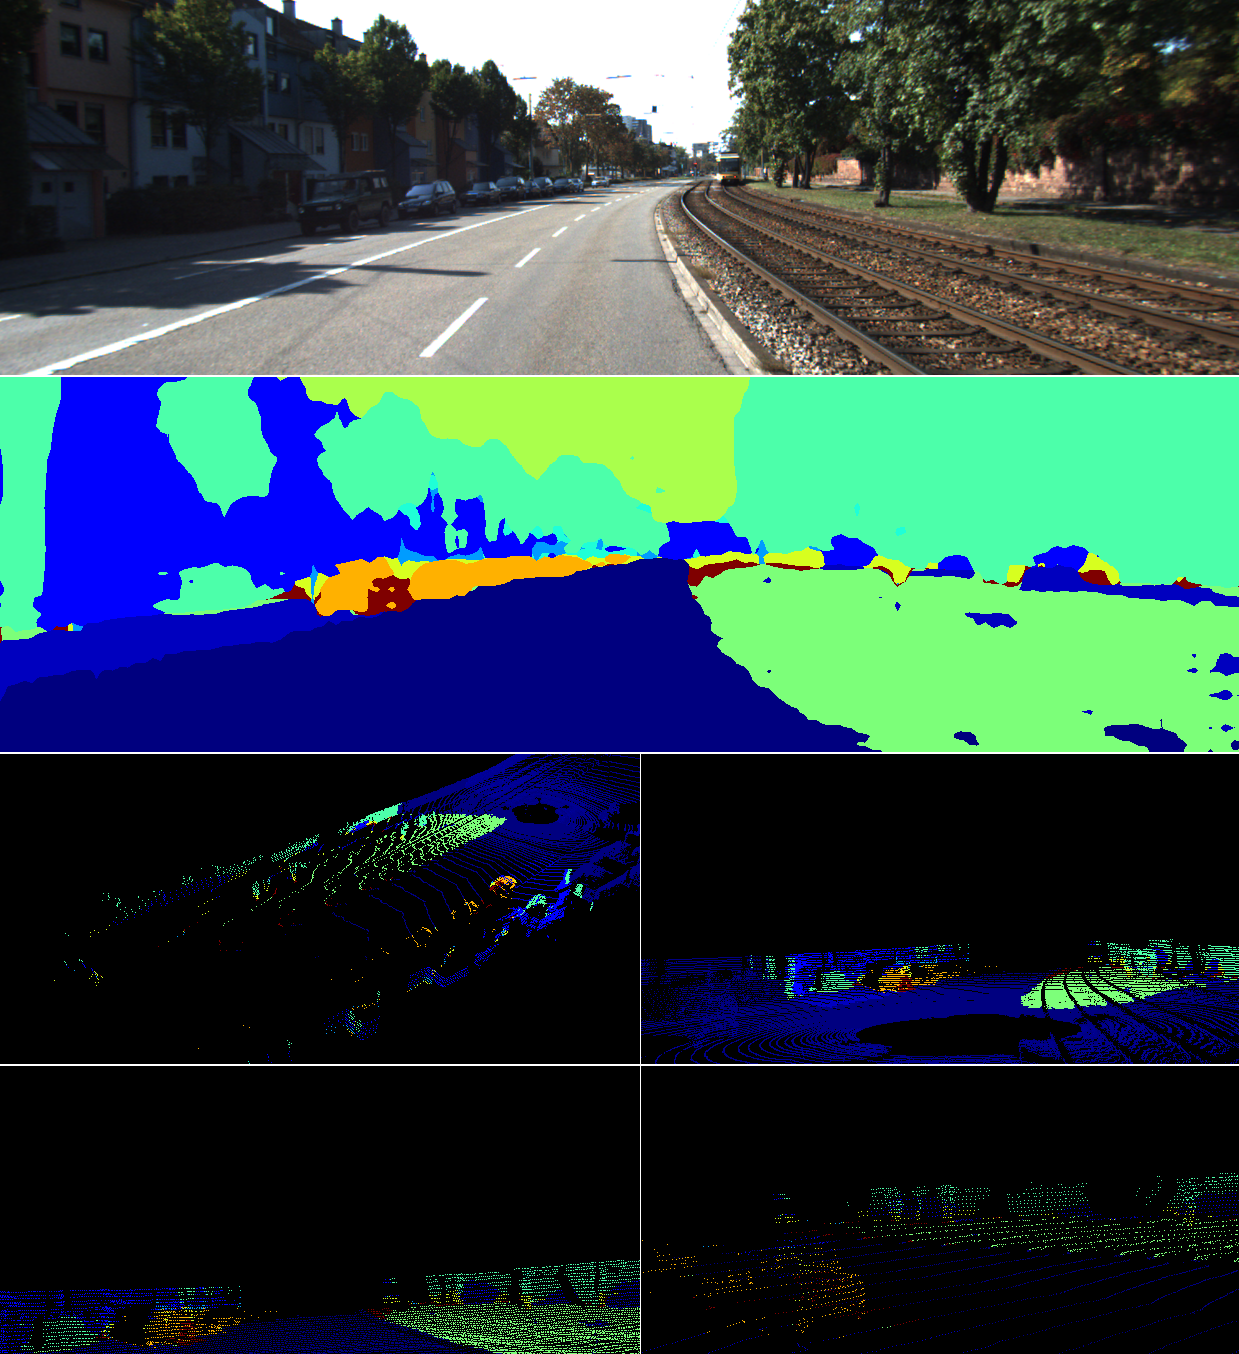
\includegraphics[width=15cm]{img/BeispielPWSegmentierung.png}
			\caption{Beispiel f�r segmentierte Punktwolke aus dem KITTI-Datensatz. Zu sehen ist von oben nach unten: Originalbild, Ergebnis von DeepLab, segmentierte Punktwolke aus verschiedenen Perspektiven.}
			\label{fig:BspPW}
		\end{figure}
   \chapter{Datens�tze}
	Methoden, die auf �berwachtes Lernen zur�ckgreifen, erfordern in der Regel eine gro�e Menge an Trainingsdaten, um verwendbare Resultate zu erzielen. Das Erstellen von Labeln f�r semantische Segmentierung ist besonders aufw�ndig, da jedem Pixel des Bildes eine Klasse zugeordnet werden muss. Deshalb werden in dieser Arbeit die �ffentlich zug�nglichen Datens�tze Cityscapes und KITTI genutzt. In dem Kapitel soll n�her auf verf�gbare Datens�tze eingegangen und erl�utert werden, weshalb diese beiden ausgew�hlt wurden.
	\section{Cityscapes}
		Cityscapes ist ein �ffentlich zug�nglicher Datensatz ausgelegt f�r Bildsegmentierung zum autonomen Fahren. Er bietet 5000 fein und 20000 grob auf Pixel-Ebene annotierte Bilder f�r semantische oder Instanz-Segmentierung. Der Satz an fein annotierten Aufnahmen, der in den Experimenten verwendet wird, ist unterteilt in einen Trainingssatz aus 2975 Bildern, einen Evaluierungssatz von 500 Bildern und einen Testsatz aus 1525 Bildern. Aufgenommen ist der Datensatz von einem Auto aus in 50 gr��tenteils deutschen St�dten, jeweils am Tag bei sonnigem oder bew�lktem Wetter um Fr�hling, Sommer und Herbst. Die Bilder zeigen ausschlie�lich Szenen, die sich auf vielbefahrenen Stra�en abspielen.\\
		Die Daten sind aufgenommen mit einer Stereo-Kamera, die hinter der Windschutzscheibe des Fahrzeugs angebracht ist, bei einer Frame-Rate von 17Hz. Die Bilder des Datensatzes sind kalibriert, Bayer-gefiltert und rektifiziert. Abbildung \ref{fig:BspCS} zeigt Beispiele.
		F�r weitere Informationen siehe \cite{Cityscapes}.\\
		\begin{figure}[h!]
			\centering
			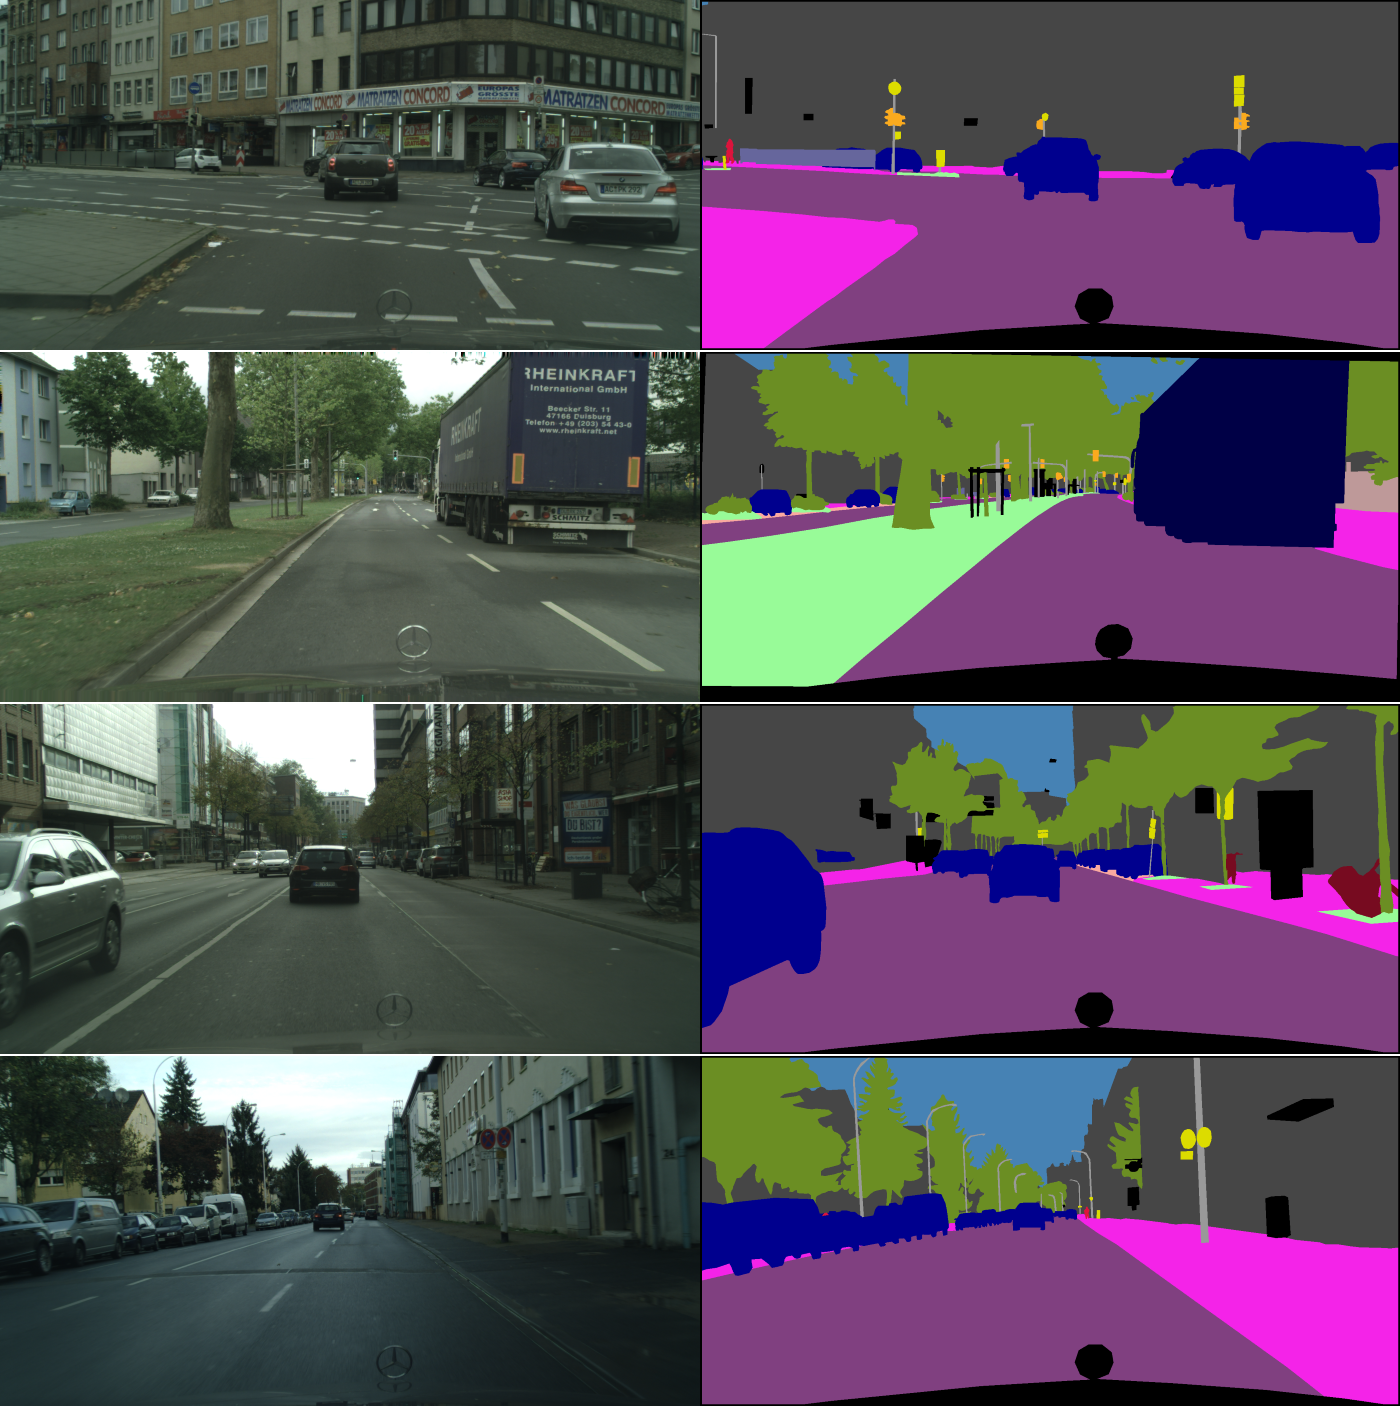
\includegraphics[width=10cm]{img/Cityscapes.png}
			\caption{Hier zu sehen sind beispielhaft fein annotierte Trainingsdaten f�r semantische Segmentierung aus dem Cityscapes-Datensatz. Wie man sieht, werden die Bilder (links) von einer hinter der Windschutzscheibe platzierten Kamera aufgenommen. Die rechte Spalte zeigt die eingef�rbte Ground Truth f�r semantische Segmentierung. Die schwarz markierten Bildfl�chen geh�ren keiner im Datensatz gelabelten Klasse an und werden w�hrend des Trainings ignoriert.}
			\label{fig:BspCS}
		\end{figure}
		Die gro�e Anzahl an qualitativ hochwertigen Bilder und Annotationen, sowie deren Verf�gbarkeit machen Cityscapes zu einer logischen Wahl f�r diese Arbeit. 
	\section{KITTI}
		Das in \cite{KITTI} beschriebene KITTI ist ein Datensatz f�r Forschung in den Bereichen mobile Robotik und autonomes Fahren. Es werden darin Kamerabilder, Laserscans, GPS- und IMU-Daten zur Verf�gung gestellt. Die Kamerabilder werden von zwei Stereo-Kamera-Rigs aufgenommen, eines f�r Farbaufnahmen, eines f�r Graustufenbilder und liegen sowohl als Rohdaten als auch rektifiziert vor. Die Laserscan-Daten sind im Velodyne LiDAR-Format gespeichert. Die Kalibrierungs-Matrizen sind im Rohdatensatz ebenfalls angegeben.\\
		Der Datensatz umfasst insgesamt 6 Stunden an Aufnahmen mit zwischen 10Hz und 100Hz aus Karlsruhe. KITTI bietet au�erdem 200 f�r Segmentierung annotierte Bilder. Die Messger�te sind auf einer mobilen Plattform auf einem Auto angebracht. Die Perspektive unterscheidet sich also geringf�gig von der der Cityscapes-Daten. F�r weitere Informationen �ber die verwendeten Messger�te siehe \cite{KITTI}.\\
		Im Gegensatz zum Cityscapes-Datensatz, der sich auf Stra�enverkehr spezialisiert, wird im KITTI-Datensatz versucht, eine m�glichst gro�e Szenenvielfalt anzubieten. Beispiele f�r Bilder des Datensatzes sind in Abbildung \ref{fig:BspKT} zu sehen. KITTI wird in dieser Arbeit verwendet, da darin, im Gegensatz zu Cityscapes, neben der Bilder Punktwolken und Projektionsmatrizen zur Verf�gung gestellt werden. Die mit Cityscapes konformen Trainingsdaten f�r semantische Segmentierung erlauben noch dazu Experimente mit der Verfeinerung des Netzes durch Nachtraining und Auswertung der vom Netz produzierten Ergebnisse mit anderen Daten als dem Cityscapes-Datensatz.
		\begin{figure}[h!]
			\centering
			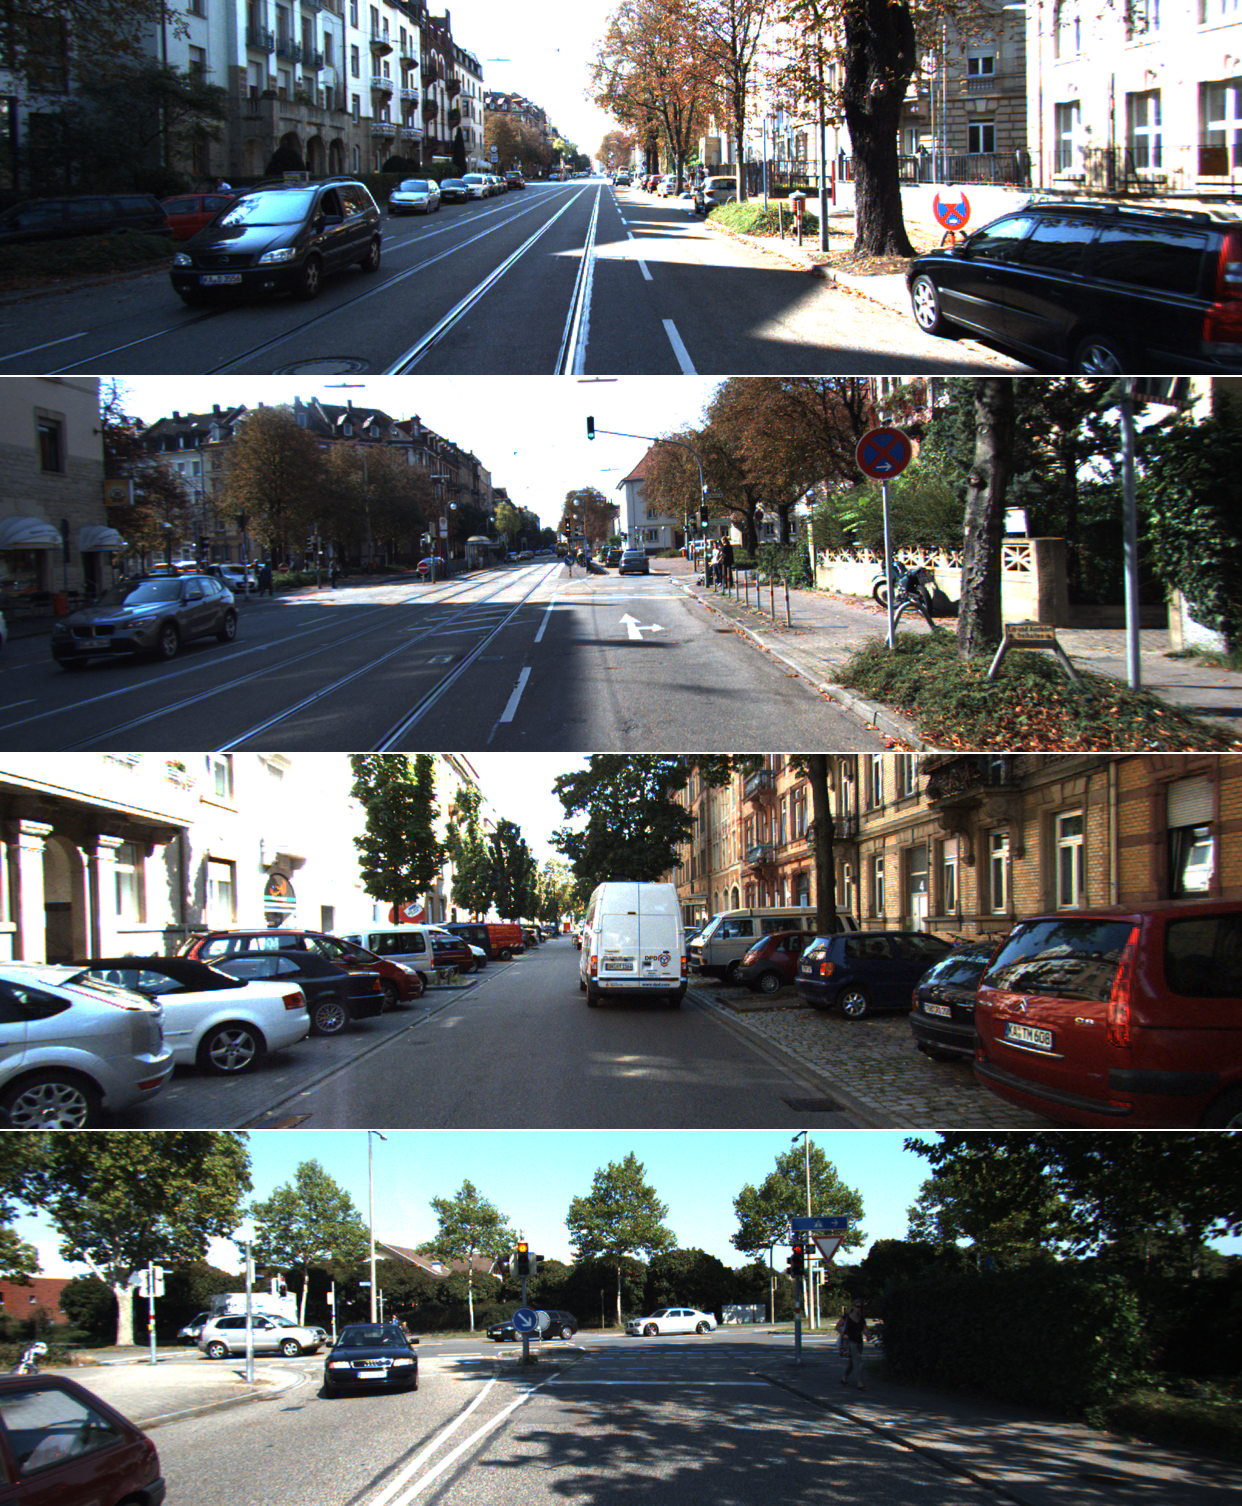
\includegraphics[width=10cm]{img/Kitti.png}
			\caption{Beispiele aus dem KITTI-Datensatz f�r semantische Segmentierung. Auf die Abbildung der Ground Truth wird verzichtet, da keine eingef�rbte Version bereitgestellt wird und es sich nicht in erster Linie um einen Datensatz f�r Segmentierung handelt. Die Bilder sind von einer mobilen Plattform aufgenommen, die sich auf dem Fahrzeug befindet, weshalb die Perspektive sich von der der Cityscapes-Daten unterscheidet.}
			\label{fig:BspKT}
		\end{figure}
	
	\section{COCO}
		Bei dem in \cite{DBLP:journals/corr/LinMBHPRDZ14} von Microsoft vorgestellten COCO (Common Objects in Context) handelt es sich um einen umfangreichen Datensatz f�r Instanz-Segmentierung. Es werden darin 328.000 Bilder mit insgesamt 2,5 Millionen annotierten Instanzen geboten. Das Bildmaterial f�r COCO stammt aus dem Internet, wobei nicht-ikonische Bilder, die Objekte aus untypischen Perspektiven zeigen, bevorzugt wurden. Da sich die Annotationen auf z�hlbare Objekte beschr�nken, ist der COCO-Datensatz f�r den Zweck dieser Arbeit nicht geeignet.
		
	\section{Pascal VOC}
		Wie in \cite{Everingham10} beschrieben, ist Pascal VOC (Visual Object Classes) eine Sammlung �ffentlich zug�nglicher Datens�tze f�r Bildklassifizierung, Objekt-Detektion, Segmentierung und Personen-Layout (Detektierung von K�rperteilen), sowie ein j�hrlicher Wettbewerb in diesen Bereichen im Zeitraum von 2007 bis 2012. Die Hauptdisziplinen sind dabei Bildklassifizierung und Objekt-Detektion. Der letzte Stand von Pascal aus dem Jahr 2012 umfasst insgesamt 11.530 Bilder mit 27.450 Region-of-Interest-annotierten Objekten und 6.929 Segmenten aus 20 verschiedenen Klassen. Die Bilder f�r die Datens�tze stammen aus dem Internet und sind ohne Pr�ferenz hinsichtlich Bildqualit�t, Perspektive, Beleuchtung und �hnlichem ausgew�hlt.\\
		In \cite{mottaghi_cvpr14} wird ein Datensatz vorgestellt, der den Anforderungen dieser Arbeit entspricht und eine valide Alternative zu Cityscapes darstellen k�nnte. Im gegebenen Kontext wird trotzdem Cityscapes verwendet wegen dessen st�rkeren Praxisbezugs und konsequenteren Label-Politik. Dazu kommt, dass Pascal Daten aus allgemeinen Szenen anbietet, w�hrend sich Cityscapes auf den Stra�enverkehr konzentriert und f�r dieses Thema leichter LiDAR-Daten gefunden werden k�nnen.
		
	\section{WildDash}
		WildDash \cite{Zendel_2018_ECCV} ist ein Datensatz, der spezifisch f�r das Testen von Methoden zur Bildsegmentierung mit Szenen aus dem Stra�enverkehr zusammengestellt ist. �hnlich wie bei KITTI ist der Satz an annotierten Bildern nicht ausreichend, um einen ad�quaten Trainingssatz zu bilden, ist aber konform mit Cityscapes und kann eine sinnvolle Erweiterung von dessen Trainingssatz darstellen.\\
		Die Bilder in WildDash stammen von "`YouTube-Autoren"' und sind nach speziellen Kriterien ausgew�hlt. Zu diesen geh�rt unter anderem, dass in den Daten Situationen gezeigt werden, die erfahrungsgem�� schwierig auszuwerten sind und potentiell Risiken darstellen, wie zum Beispiel Tiere auf der Fahrbahn und Tunnelausfahrten. Au�erdem enth�lt der Datensatz negative Testf�lle, also Bilder bei denen ein schlechtes Ergebnis erwartet wird, wie beispielsweise gedrehte Bilder.\\
		Im Rahmen dieser Arbeit wird der KITTI-Datensatz als geeigneter angesehen, da darin auch Punktwolken gestellt und haupts�chlich st�dtische Szenen gezeigt werden. Au�erdem erscheinen Testergebnisse auf den bewusst problematischen Daten aus dem WildDash-Datensatz weniger repr�sentativ.
		
		
   \chapter{Experimente}
	\section{Technische Daten des f�r die Experimente verwendeten Rechners}
		\begin{itemize}
			\item Prozessor: Intel(R) Core(TM) i7-7700HQ CPU @ 2.860GHz
			\item Grafikkarte: NVIDIA GeForce GTX 1070
			\item Arbeitsspeicher: 16GB RAM
		\end{itemize}
	\section{Backbones}
		F�r die Durchf�hrung folgender Experimente wird der fein annotierte Cityscapes-Datensatz verwendet. Die Netze werden auf dem aus 2975 Bildern bestehenden Trainingssatz trainiert und auf dem 500 Bilder fassenden Validierungssatz ausgewertet.\\
		F�r jede Trainingsepoche werden aus dem Trainingssatz 1487 Bilder zuf�llig ausgew�hlt. Als Grundlernrate wird 0.007 gew�hlt. Der Trainingsfehler wird �ber die in \cite{Lovasz} beschriebene Lovasz-Funktion berechnet. Weitere Hyperparameter sind eine Dropout-Rate von 0.1,  eine L2 Regularisierungsrate von $4*10^{-5}$ und ein Momentum-Faktor von 0.9.\\
		Die Netzwerkausgaben werden mittels der im Bereich Bildsegmentierung �blichen Intersection-over-union-Metrik (IoU) ausgewertet, die sich folgenderma�en berechnet:\\
		\begin{equation}
			IoU = \frac{TP}{TP + FP + FN}
		\end{equation}
		Dabei steht TP f�r True Positives, also richtig erkannte Pixel, FP f�r False Positives und FN f�r False Negatives. Da in diesem System jedem  Pixel eine g�ltige Klasse zugeordnet wird, sind FP und FN hier stets identisch.
		
		\subsection{MobileNetV2}
			\label{sec:mn2}
			Da Echtzeitf�higkeit eine wichtige Rolle spielt, konzentrieren sich die Experimente auf das leichtgewichtige MobileNetV2, statt dem leistungsf�higeren Xception65. Das erste Experiment besch�ftigt sich mit dem Finden der idealen Trainingsdauer.
			%\subsubsection{Auswirkungen der Trainingsdauer}
			\begin{table}[h]
				\centering
				\begin{tabular}{l|cccccc}
					Epochen trainiert & 1 & 5 & 10 & 15 & 25 & 30\\\hline
					IoU Stra�e & 0.6260 & 0.6498 & 0.6727 & 0.6729 & 0.6774 & 0.6675\\\hline
					IoU Gehsteig & 0.1835 & 0.3788 & 0.4330 & 0.4616 & 0.5193 & 0.5078\\\hline
					IoU Geb�ude & 0.5563 & 0.6402 & 0.6573 & 0.6771 & 0.6931 & 0.7068\\\hline
					IoU Mauer & 0.0 & 0.0 & 0.0 & 0.0 & 0.0 & 0.0\\\hline
					IoU Zaun & 0.0 & 0.0 & 0.0 & 0.0 & 0.0 & 0.0\\\hline
					IoU Pfahl & 0.0791 & 0.1931 & 0.2159 & 0.2561 & 0.2835 & 0.2728\\\hline
					IoU Ampel & 0.0 & 0.0 & 0.0 & 0.0 & 0.0 & 0.0\\\hline
					IoU Verkehrszeichen & 0.0 & 0.1056 & 0.1785 & 0.1859 & 0.2233 & 0.2291\\\hline
					IoU Vegetation & 0.5581 & 0.7153 & 0.7273 & 0.7518 & 0.7728 & 0.7663\\\hline
					IoU Gel�nde & 0.0 & 0.0915 & 0.1274 & 0.1355 & 0.1593 & 0.1445\\\hline
					IoU Himmel & 0.5353 & 0.6606 & 0.6867 & 0.6977 & 0.7153 & 0.7081\\\hline
					IoU Person & 0.0 & 0.1160 & 0.1582 & 0.1458 & 0.1680 & 0.1863\\\hline
					IoU Radfahrer & 0.0 & 0.0 & 0.0 & 0.0 & 0.0 & 0.0\\\hline
					IoU Auto & 0.3537 & 0.5438 & 0.6014 & 0.5863& 0.6419 & 0.6103\\\hline
					IoU Lastwagen & 0.0 & 0.0 & 0.0 & 0.0 & 0.0 & 0.0\\\hline
					IoU Bus & 0.0 & 0.0 & 0.0 & 0.0 & 0.0 & 0.0\\\hline
					IoU Zug & 0.0 & 0.0 & 0.0 & 0.0 & 0.0 & 0.0\\\hline
					IoU Motorrad & 0.0 & 0.0 & 0.0 & 0.0 & 0.0 & 0.0\\\hline
					IoU Fahrrad & 0.0 & 0.0 & 0.0 & 0.0750 & 0.1340 & 0.1542\\\hline
					Durchschnitt IoU & 0.1522 & 0.2155 & 0.2346 & 0.2444 & 0.2625 & 0.2607\\\hline
					Durchschnitt IoU $\neq 0$ & 0.4131 & 0.4094 & 0.4458 & 0.4222 & 0.4534& 0.4503\\
					
						
				\end{tabular}
				\caption{Die Tabelle zeigt die Bewertung von Models in Intersection-over-union (IoU) Metrik in Abh�ngigkeit der Trainingsdauer.}
				\label{lbl: IoUs}
			\end{table}
		
			\begin{figure}[h]
				\centering
				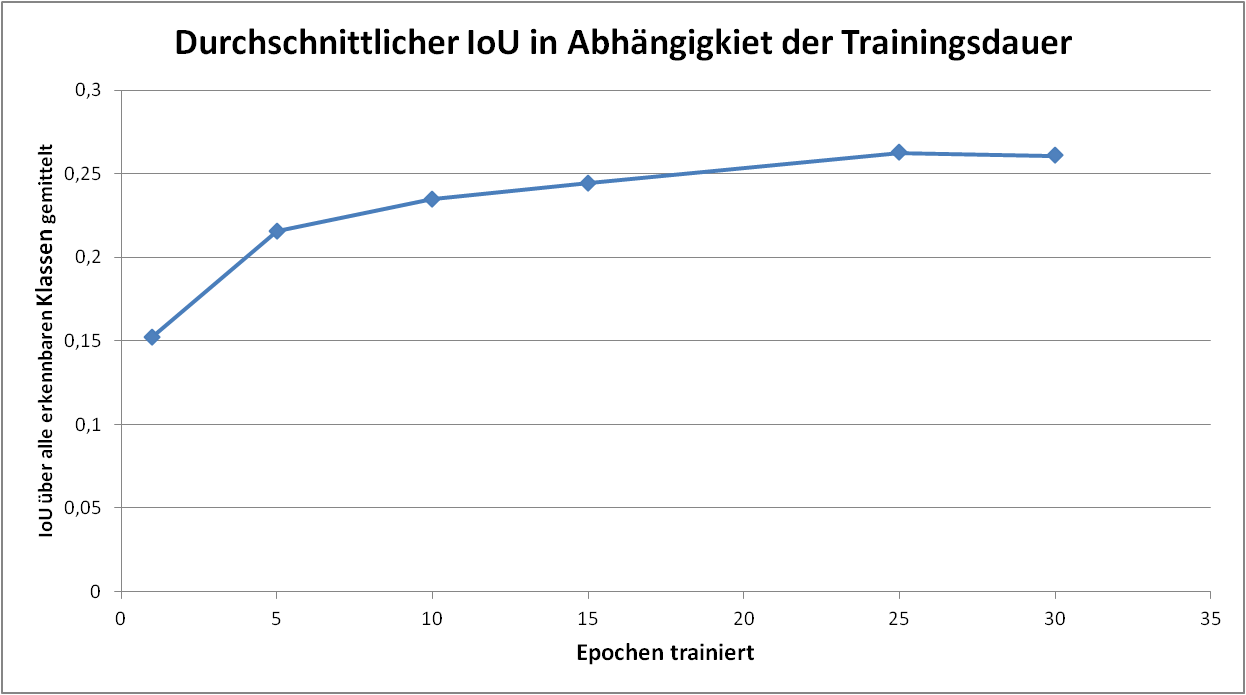
\includegraphics[width=15cm]{img/IoUMobilenet.png}
				\caption{Durchschnittlicher IoU in Abh�ngigkeit der Anzahl trainierter Epochen. Der Graph erreicht sein Maximum bei 25 Epochen und f�llt danach leicht ab, was auf Overfitting schlie�en l�sst.}
				\label{fig:IoUMn}
			\end{figure} 
		
			Wie in Tabelle \ref{lbl: IoUs} und Abbildung \ref{fig:IoUMn} zu erkennen ist, verbessert sich die Bewertung des Models bis zu einem Punkt, der in etwa bei Epoche 25 liegt und verschlechtert sich bei Verl�ngerung der Trainingsdauer wieder. Es tritt also trotz der L2 Regularisierung der Netzparameter und der Nutzung des Dropout-Verfahrens wahrscheinlich Overfitting auf. Im Folgenden wird das f�r 25 Epochen trainierte Netz verwendet. Die Bewertung dieses Models ist in Abbildung \ref{fig:KIoUMn} dargestellt.\\
			
			\begin{figure}
				\centering
				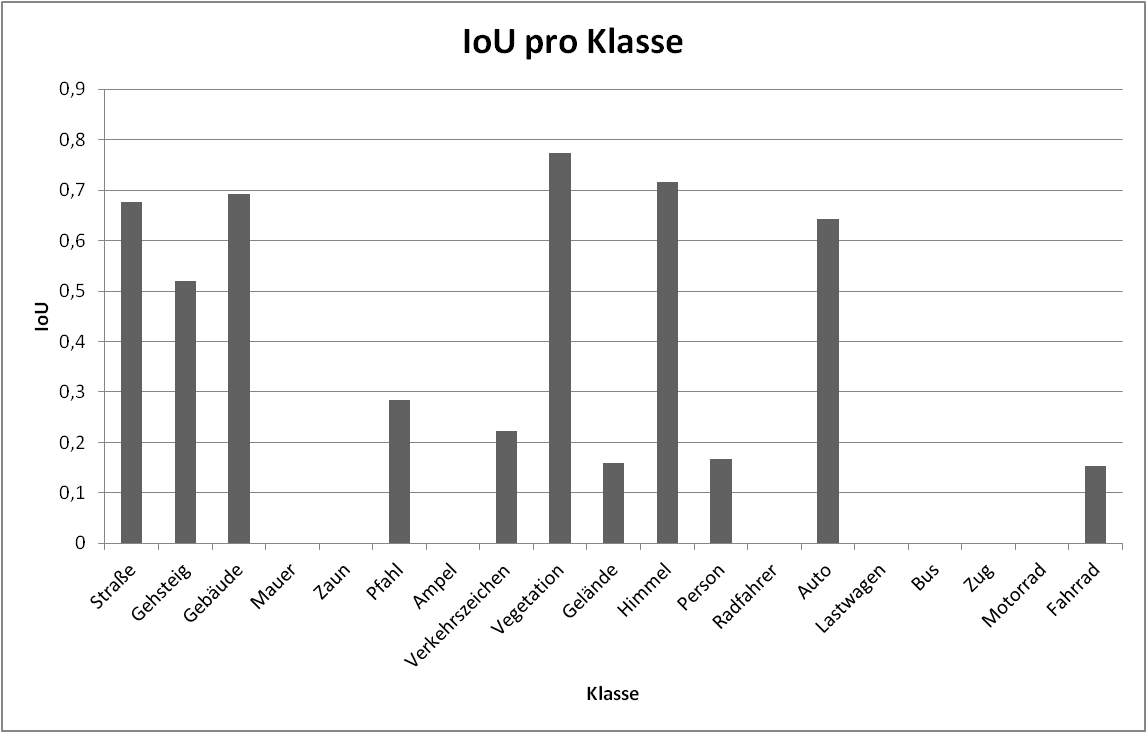
\includegraphics[width=15cm]{img/KlasseIoUMobilenet.png}
				\caption{IoU f�r jede Klasse vom Test des f�r 25 Epochen trainierten Netzes. Das Diagramm zeigt gute Ergebnisse f�r amorphe Klassen und schlechtere f�r kleine Objekte. Zu sehen ist auch, dass einige Klassen, die in den Trainingsdaten selten vorkommen oder �hnlichkeit mit anderen Klassen aufweisen, nicht erkannt werden.}
				\label{fig:KIoUMn}
			\end{figure} 
		
			Die Models weisen durchwegs ihre h�chsten Ergebnisse beim Erkennen der amorphen Klassen Stra�e, Geb�ude, Vegetatio und Himmel auf, wie bei einem semantischen Segmentierungsverfahren zu erwarten. Das niedrige Ergebnisse bei der Klasse Gel�nde l�sst sich dadurch erkl�ren, dass der Cityscapes-Datensatz in st�dtischen Umgebungen aufgenommen wird, wo diese Klasse selten auftritt. Vergleichsweise hoch ist auch der IoU-Wert f�r die Klasse Auto, die in dem Datensatz besonders h�ufig ist.\\
			Die niedrigsten positiven IoU-Werte weisen die Ergebnisse bei kleineren, z�hlbaren Objekten wie Personen, Pf�hle, Fahrr�der und Verkehrszeichen auf. \\
			Die in Abbildung \ref{fig:KIoUMn} dargestellten Ergebnisse lassen au�erdem erkennen, dass das Netz bestimmte Klassen praktisch nicht erkennt. Dies l�sst vermuten, dass es nur eingeschr�nkt f�hig ist, Bildsegmente anhand ihres Kontextes zu bewerten und beispielsweise zwischen einem Fu�g�nger und einem Fahrradfahrer oder zwischen einer Mauer und einem Geb�ude zu unterscheiden und die h�ufiger auftretende Variante ausw�hlt. Die Ergebnisse der Klasse Fahrrad lassen vermute, dass ein l�ngeres Training dieses Verhalten verbessern k�nnte. Da ein zu langes Training sich, wie vorher erw�hnt, negativ auf den durchschnittlichen IoU auswirkt, wird in diesem Experiment aber davon abgesehen. Eine weitere M�glichkeit w�re, dem Trainingssatz mehr Daten hinzuzuf�gen, die vermehrt die entsprechenden Objekte enthalten.\\
			
			\begin{figure}
				\centering
				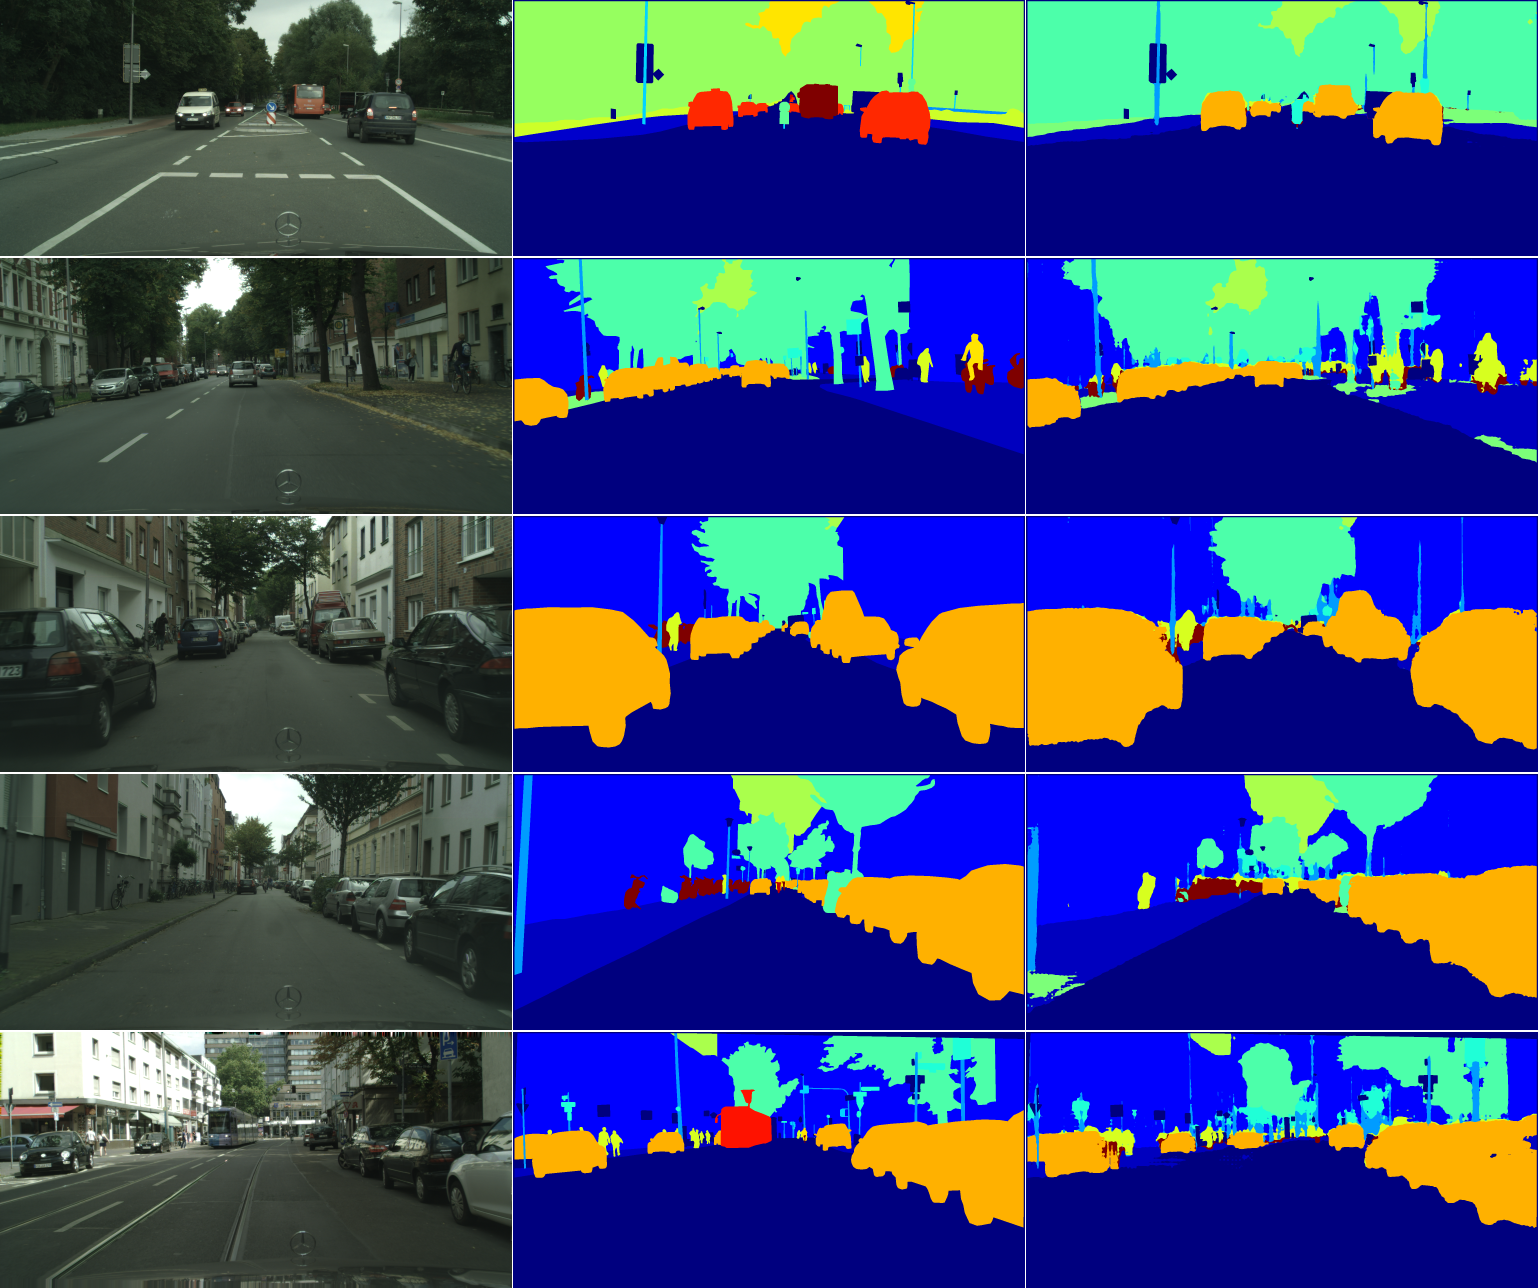
\includegraphics[width=15cm]{img/BeispielMobilenet.png}
				\caption{Zu sehen sind Beispiele f�r Ausgaben des Models mit der besten Bewertung im vorherigen Experiment (25 Epochen trainiert).\\ Von links nach rechts gezeigt sind Eingabebild, Ground Truth, Ausgabe von DeepLab.}
				\label{fig:BspMn}
			\end{figure} 
			
			Abbildung \ref{fig:BspMn} zeigt ausgew�hlte Ausgaben des f�r 25 Epochen lang trainierten Netzes, das die besten Ergebnisse in der IoU-Metrik liefert. Sie spiegeln die Bewertung aus Tabelle \ref{lbl: IoUs} wieder, mit hoher Genauigkeit bei gro�en und amorphen Objekten und niedriger bei kleineren, z�hlbaren. Besonders auff�llig sind False Positives der Klasse Person, die das Model oft an Fahrr�der oder B�ume in der n�he von Personen vergibt.\\
			Die Beispiele lassen erkennen, dass das Netz teilweise die Trainingsdaten memorisiert. So wird dem oberen Teil eines Fahrrades h�ufig die Klasse Person zugewiesen und umgekehrt der untere Teil einer Person als Fahrrad erkannt. Genauso werden Bereiche, die sich �ber einem als Stra�e erkannten Segments befinden tendenziell eher als Auto klassifiziert. Das l�sst sich auf die Funktion des CRF zur�ckf�hren.
		
	\subsection{Xeption65}
		Wir betrachten den Xception65-Backbone im Vergleich zu MobileNetV2. Auf ein Experiment mit unterschiedlichen Trainingsepochen wird an dieser Stelle aufgrund der langen Trainingsdauer der Netze verzichtet. Das verwendete Model ist 60 Epochen lang trainiert mit denselben Hyperparametern wie die Models mit MobileNetV2.
		
		\begin{table}[h]
			\centering
			\begin{tabular}{l|cc|c}
				 & Xception65 & MobileNetV2 &  Differenz \\\hline
				IoU Stra�e & 0.6951 & 0.6774 & 0.0177 \\\hline
				IoU Gehsteig & 0.7238 & 0.5193 & 0.2045 \\\hline
				IoU Geb�ude & 0.8533 & 0.6931 & 0.1602 \\\hline
				IoU Mauer & 0.1461 & 0.0 & 0.1461 \\\hline
				IoU Zaun & 0.1641 & 0.0 & 0.1641 \\\hline
				IoU Pfahl & 0.5843 & 0.2835 & 0.3008 \\\hline
				IoU Ampel & 0.3049 & 0.0 & 0.3049 \\\hline
				IoU Verkehrszeichen & 0.6592 & 0.2233 & 0.4359 \\\hline
				IoU Vegetation & 0.8558 & 0.7728 & 0.0830 \\\hline
				IoU Gel�nde & 0.2068 & 0.1593 & 0.0475 \\\hline
				IoU Himmel & 0.7707 & 0.7153 & 0.0554 \\\hline
				IoU Person & 0.5234 & 0.1680 & 0.3554 \\\hline
				IoU Radfahrer & 0.2386 & 0.0 & 0.2386 \\\hline
				IoU Auto & 0.8369 & 0.6419 & 0.1950 \\\hline
				IoU Lastwagen & 0.0691 & 0.0 & 0.0691 \\\hline
				IoU Bus & 0.0893 & 0.0 & 0.0893 \\\hline
				IoU Zug & 0.0185 & 0.0 & 0.0185 \\\hline
				IoU Motorrad & 0.0685 & 0.0 & 0.0685 \\\hline
				IoU Fahrrad & 0.4080 & 0.1340 & 0.4080 \\\hline
				Durchschnitt IoU & 0.4324 & 0.2625 & 0.2346 \\\hline
				Durchschnittliche & 764 & 387 & 377 \\
				Verarbeitungszeit [ms] & & & \\
				
			\end{tabular}
			\caption{Gezeigt ist ein Vergleich zwischen den Ergebnissen von DeepLab mit Xception65 und MobileNetV2 in IoU-Metrik und der Verarbeitungszeit.}
			\label{lbl: XcVsMn}
		\end{table}
	
		\begin{figure}
			\centering
			\includegraphics[width=15cm]{img/XceptionVsMobileNet.png}
			\caption{Der Vergleich von Xception65 und MobileNetV2 in IoU-Metrik zeigt, dass Xception die besten Ergebnisse bei denselben Klassen wie MobileNetV2 produziert, aber deutlich besser beim Erkennen von Objekten und Details ist.}
			\label{fig:XcVsMn}
		\end{figure} 
		
		Wie in Tabelle \ref{lbl: XcVsMn} und Abbildung \ref{fig:XcVsMn} zu sehen ist, erzeugt das Model mit Xception65 durchwegs bessere Ergebnisse als das mit MobileNetV2, ben�tigt aber im Durchschnitt 97\% mehr Zeit f�r die Verarbeitung eines Eingabebildes.\\
		Durch die Verwendung von Xception65 ist das Model au�erdem in der Lage, alle Klassen des Datensatzes zu erkennen, auch wenn die IoU-Werte f�r die von MobileNetV2 nicht erkannten Klassen vergleichsweise niedrig sind. Eine besonders gro�e Steigerung der Bewertung im Vergleich mit MobileNetV2 weist das Netz bei kleineren, z�hlbaren Objekten auf wie Personen (311\%) und Verkehrszeichen (295\%) auf.\\
		Abbildung \ref{fig:BspXc} zeigt beispielhafte Ergebnisse des Models aus dem Validierungs-Datensatz von Cityscapes.
		
		\begin{figure}[h]
			\centering
			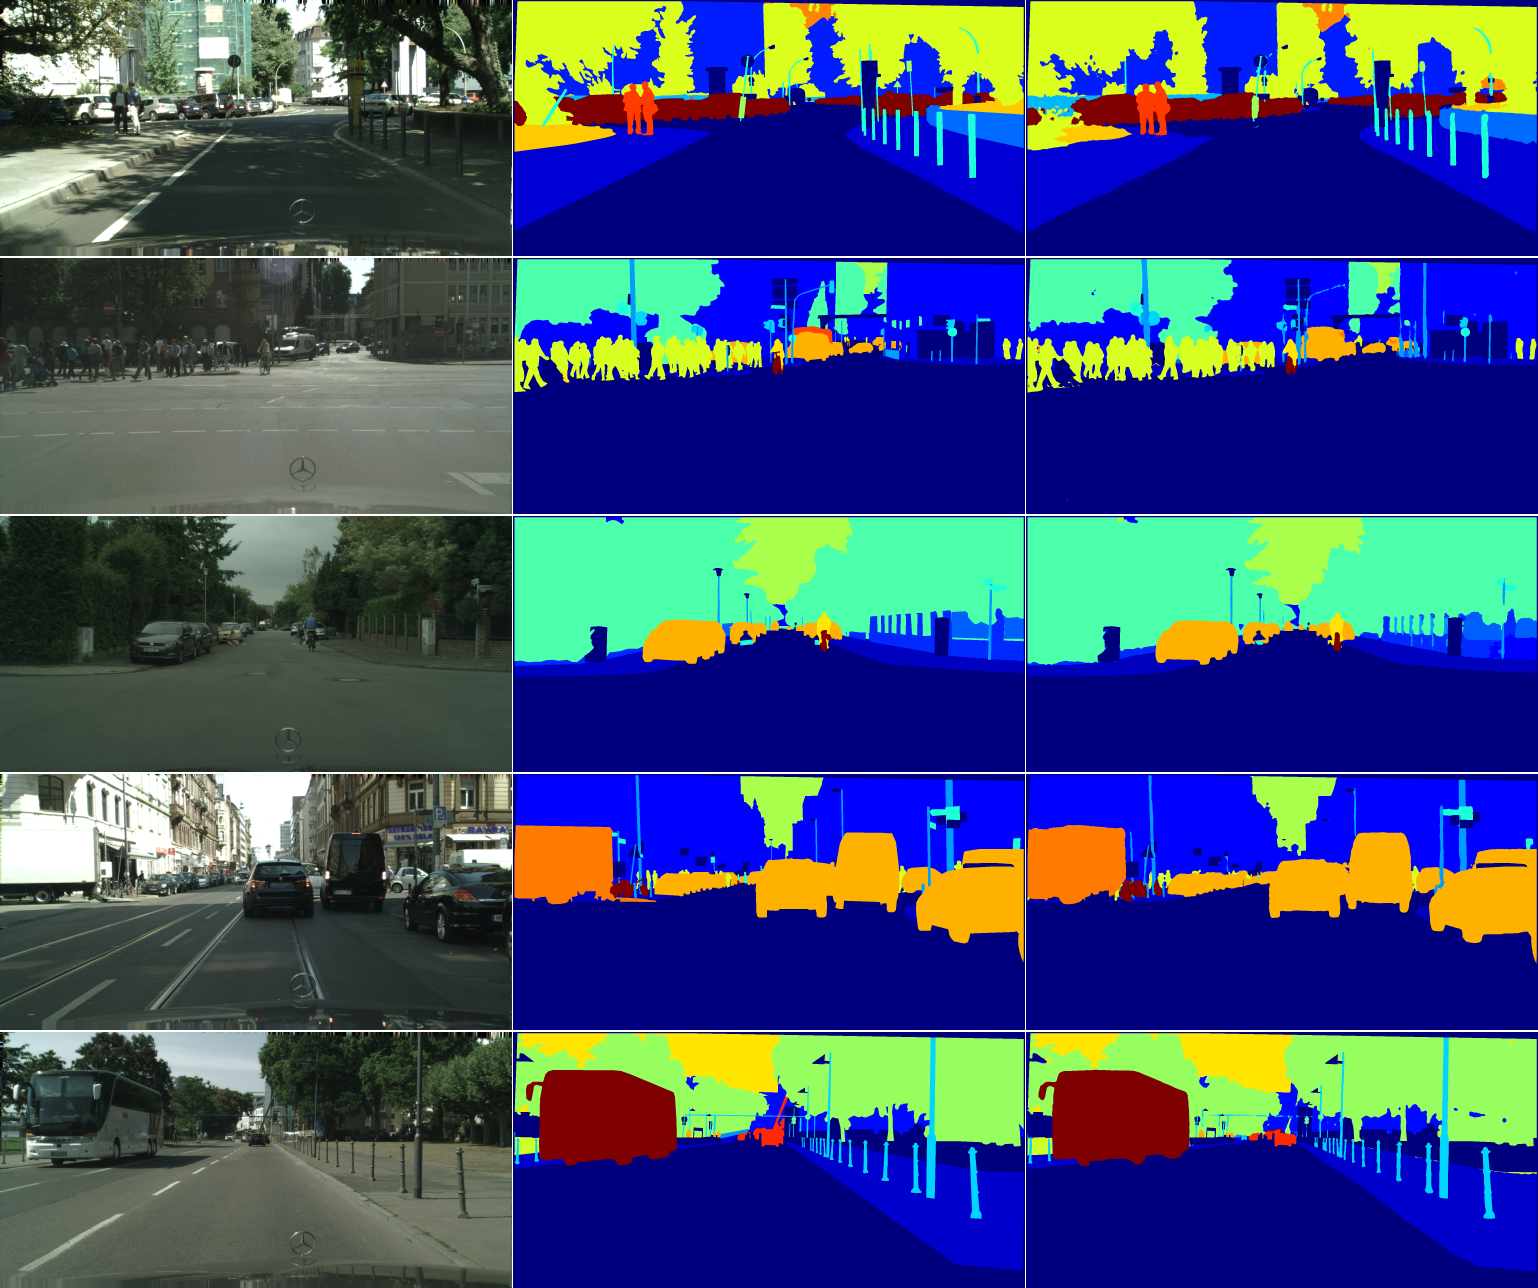
\includegraphics[width=15cm]{img/BeispielXception.png}
			\caption{Gezeigt sind Beispiele f�r Ausgaben des Models, das Xception65 nutzt.\\ Von links nach rechts zu sehen ist Eingabebild, Ground Truth, Ausgabe von DeepLab.}
			\label{fig:BspXc}
		\end{figure} 
		
		
		
	\section{Verfeinerung mit KITTI}
		In diesem Experiment wird das am besten bewertete, mit Cityscapes trainierte Model mit MobileNetV2 als Backbone mehrere Epochen mit den 200 Bildern umfassenden Trainingsdaten f�r semantische Segmentierung von KITTI nachtrainiert. Die Resultierenden Models werden anschlie�end mit anderen Bildern aus dem KITTI-Datensatz getestet. Da KITTI nur f�r diese 200 Bilder eine Ground Truth zur Verf�gung stellt und ein Test auf den Trainingsdaten wenig aussagekr�ftig ist, begn�gt sich das Experiment in diesem Fall mit einer empirischen Auswertung.\\
		Abbildung \ref{fig:Verf} zeigt beispielhaft je ein Bild aus beiden Datens�tzen und die Ausgaben von DeepLab f�r verschieden lang nachtrainierte Models.  
		\begin{figure}[h]
			\centering
			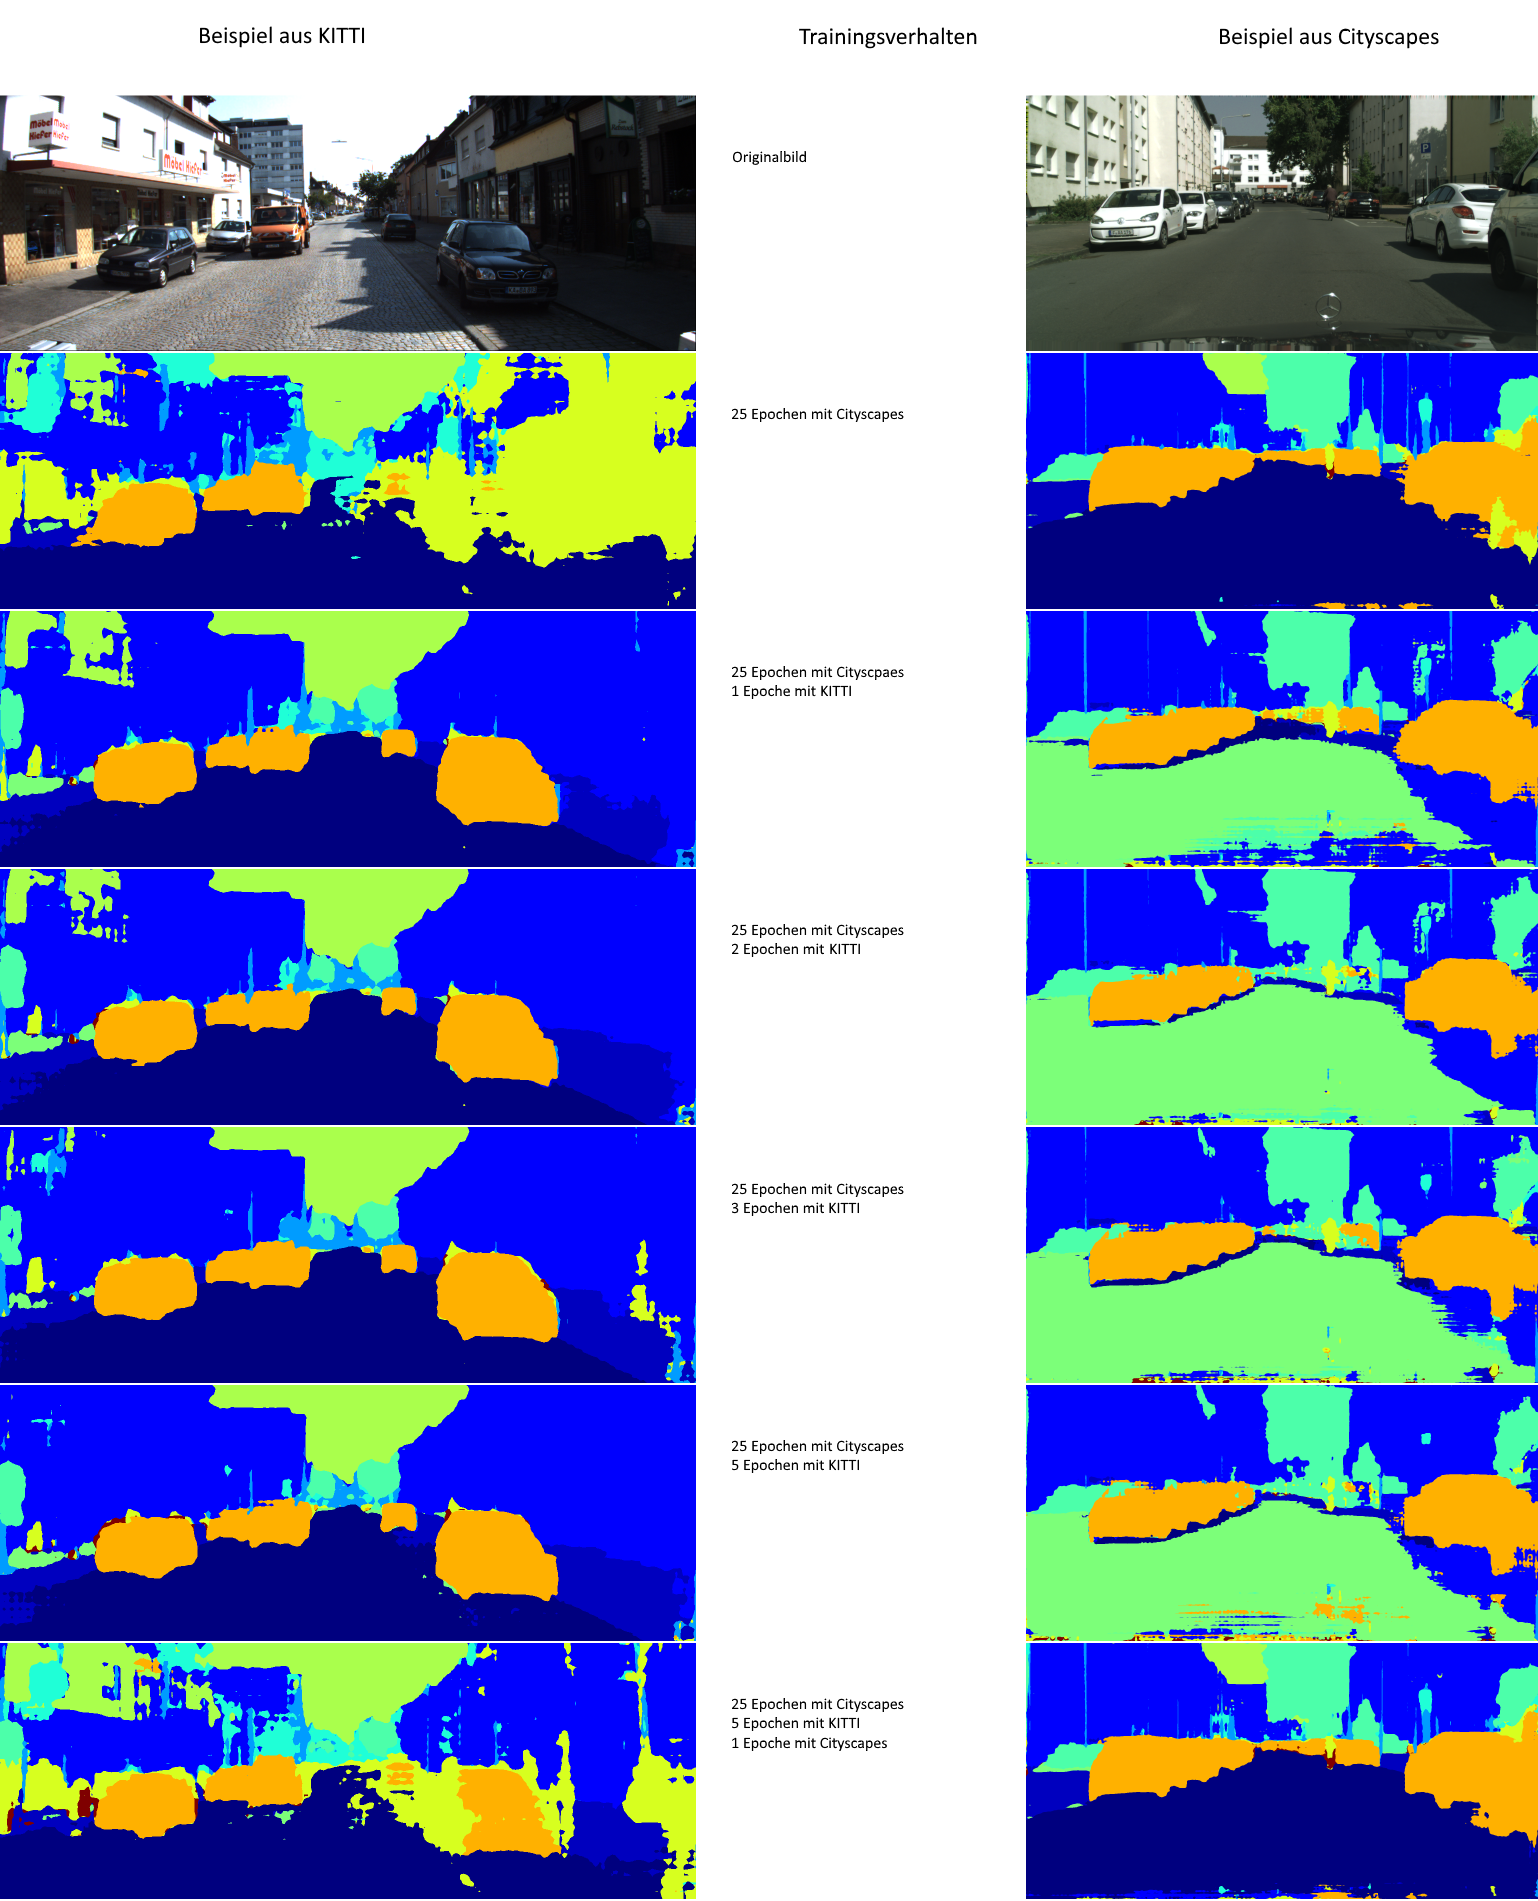
\includegraphics[width=15cm]{img/Verfeinerung.png}
			\caption{Beispiel f�r Ausgabe von mit KITTI-Daten verfeinerter Models. Die erste Epoche der Verfeinerung zeigt die gr��te Verbesserung auf den KITTI-Daten und gleichzeitig eine deutliche Verschlechterung bei Cityscapes-Bildern. Dieses Verhalten ist durch ein Nachtraining mit Cityscapes reversibel. Das Experiment zeigt, dass Overfitting ein Problem des Netzes ist.}
			\label{fig:Verf}
		\end{figure} 
		Wie man sieht, tritt bei den Ergebnissen auf dem KITTI-Datensatz bereits nach einer Epoche Verfeinerung mit KITTI-Daten eine deutliche Verbesserung auf. Weitere Trainingsepochen verbessern die Ergebnisse weiter, aber weniger erheblich. Gleichzeitig verschlechtert sich die Ausgabe f�r ein Bild aus dem Cityscapes-Datensatz in �hnlichem Ma�e. \\Das unterste Bild von Abbildung \ref{fig:Verf} zeigt die Ausgabe eines Models, das f�r 25 Epochen auf Cityscapes-Daten trainiert, f�r 5 Epochen mit KITTI-Daten verfeinert und anschlie�end f�r eine Epoche mit Cityscapes-Daten nachtrainiert ist. Wie man sieht, f�hrt die Verfeinerung mit dem urspr�nglichen Datensatz wieder zu einer Verschlechterung der Ergebnisse auf KITTI-Bildern und einer Verbesserung auf Cityscapes-Bildern.\\
		Diese Beobachtungen best�rken die Vermutung, dass beim Trainieren des Netzes Overfitting auftritt.\\
		
		In einem n�chsten Schritt soll untersucht werden, wie die Ber�cksichtigung der KITTI-Daten beim gesamten Lernprozess die Ergebnisse auf beiden Datens�tzen beeinflusst. Dazu wird der annotierte KITTI-Datensatz geteilt in einen Trainings- und Evaluierungssatz zu je 100 Bildern. Dadurch wird es m�glich, eine Aussagekr�ftige Bewertung in IoU-Metrik zu berechnen. Aufbauend auf dem vorherigen Experiment wird ein Model mit gemischten Daten f�r 24 Epochen trainiert und ausgewertet. Danach wird es f�r eine Epoche ausschlie�lich mit KITTI-Daten verfeinert und dann f�r eine weitere Epoche mit dem gesamten, gemischten Trainingssatz nachtrainiert. Damit ist das letzte Model 25 Epochen auf den gemischten Daten trainiert und hat damit genauso viele Lernschritte auf Cityscapes-Bilder absolviert wie das am besten Bewertete Model von Abschnitt \ref{sec:mn2}. Die Ergebnisse sind in Tabelle \ref{res:mix} eingetragen. 
		 
		\begin{table}
			\centering
			\begin{tabular}{p{4cm}|m{3cm}m{3cm}}
				
				& Durchschnittlicher IoU & Durchschnittlicher IoU \\
				Trainingsverhalten&  auf Cityscapes-Bildern & auf KITTI-Bildern\\\hline
				25 Epochen mit Cityscapes-Daten & 0.2625 & 0.1681\\\hline
				24 Epochen mit gemischten Daten & 0.2605 & 0.2002\\\hline
				24 Epochen mit gemischten Daten + 1 Epoche mit KITTI-Daten & 0.2045 & 0.2350\\\hline
				24 Epochen mit gemischten Daten + 1 Epoche mit KITTI-Daten + 1Epoche mit gemischten Daten & 0.2718 & 0.2105
				
				
			\end{tabular}
			\label{res:mix}
			\caption{Die Tabelle zeigt die Bewertung von Netzwerken mit unterschiedlich verfeinerten Trainingsdaten und -verhalten auf Evaluierungss�tzen von Cityscapes und KITTI.}
		\end{table}
		
	\section{Aufgetretene Probleme und L�sungen}
		\subsection{False Positives}
			Models, die MobileNetV2 benutzen neigen dazu, einige Klassen zum Gro�teil mit einer anderen zu klassifizieren. Beispiele daf�r sind die bereits angesprochene Erkennung von Fahrr�dern als Personen und die Klassifizierung gro�er Fahrzeuge als Geb�ude. \\
			Bei Verwendung des Xception65-Backbones kommt es reproduzierbar bei bestimmten Bildern zu einem Ph�nomen, bei dem eine gro�e Anzahl Pixel nahe einer der Ecken als Stra�e beziehungsweise die Klasse mit dem niederwertigsten Label klassifiziert wird. Es besteht kein erkennbarer Zusammenhang zwischen den Bildern, bei denen dieses Verhalten auftritt. Abbildung \ref{fig:BspBadXc} zeigt Beispiele daf�r.
			\begin{figure}
				\centering
				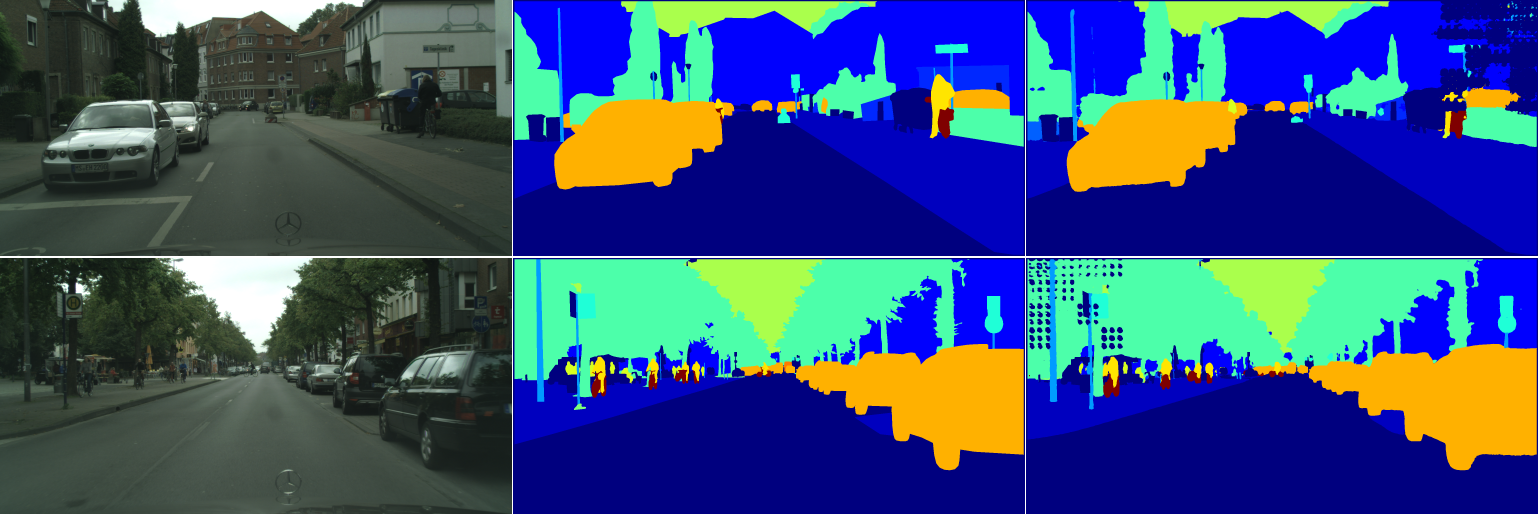
\includegraphics[width=15cm]{img/BeispielBadXception.png}
				\caption{Hier zu sehen sind Beispiele f�r Ausgaben des Models mit Xception65, die das oben beschriebene Ph�nomen aufweisen.\\ Von links nach rechts gezeigt sind Eingabebild, Ground Truth, Ausgabe von DeepLab. Das Verhalten ist auf den jeweiligen Bildern reproduzierbar.}
				\label{fig:BspBadXc}
			\end{figure} 
		\subsection{Overfitting}
			Overfitting hat sich als eines der haupts�chlichen Probleme bei der Verwendung von MobileNetV2 herausgestellt. Schon kleine �nderungen in der Perspektive, wie sie beispielsweise im KITTI-Datensatz auftritt, verursachen eine sp�rbare Verschlechterung der Ergebnisse. \\
			Um bessere Ergebnisse auf dem KITTI-Datensatz zu erzeugen, hat es sich als vorteilhaft herausgestellt, den Trainingssatz f�r semantische Segmentierung der KITTI-Daten beim Trainieren des Netzes mitzuber�cksichtigen. Das Netz mit jenen Daten nachzutrainieren verbessert ebenfalls die Ergebnisse, kann aber wiederum zu Overfitting auf diesen Datensatz f�hren. Es kann hilfreich sein, nach dem Nachtraining noch eine Epoche mit allen verf�gbaren Daten nachzutrainieren.\\
			Weitere M�glichkeiten, gegen Overfitting vorzugehen, mit denen in dieser Arbeit aber nicht experimentiert wird, sind eine Erh�hung der Dropout-Rate und dem L2 Regularisierungsfaktor.
   \chapter{Zusammenfassung}
	Ziel der Arbeit war die Entwicklung eines Systems zur semantischen Segmentierung von Bildern und Punktwolken mit neuronalen Netzen. Es soll also jedem Pixel eines Bildes, beziehungsweise jedem Punkt einer Punktwolke eine Klasse zugeteilt werden, ohne zwischen Instanzen von z�hlbaren Objekten zu unterscheiden wie das bei Instanz- oder panoptischer Segmentierung der Fall w�re.\\
	Als Netzarchitektur wurde das von Google entwickelte DeepLab verwendet. Dabei handelt es sich um ein Deep Fully-Convolutional Neural Network, das durch das Adaptieren von Atrous Convolution, Atrous Spatial Pyramid Pooling un Conditional Random Fields auf den Bereich der semantischen Bildsegmentierung angepasst ist.\\
	Wegen der Anforderungen an die Laufzeit wurde als Backbone das leichtgewichtige MobileNetV2 gew�hlt, das in Experimenten mit dem Leistungsf�higeren Xception65 verglichen wurde. Beide Netze sind als Residual Networks strukturiert, was bedeutet, dass �ber so genannte Rasidual Connections Daten �ber mehrere Verarbeitungsschichten hinweg unver�ndert weitergeleitet und auf die Ergebnisse der �bersprungenen Schichten addiert werden. Dadurch wird verhindert, dass ein Hinzuf�gen weiterer Schichten die Ergebnisse verschlechtert. Eine weitere Technik, die beide Architekturen verwenden ist Depthwise Separable Convolution, bei der zuerst eine r�umliche und dann eine dimensions�bergreifende Faltung durchgef�hrt wird. MobileNetV2 zeichnet sich durch die Verwendung von Bottleneck-Bl�cken aus. Darin werden die Daten zuerst Expandiert, dann Komprimiert, um Speicherplatz zu sparen.\\
	Da diese Arbeit das Ziel hat, Algorithmen f�r Autonomes Fahren zu unterst�tzen und verbessern, wurde die Implementierung mit Hilfe der Datens�tze Cityscapes und KITTI ausgewertet, die explizit f�r diesen Bereich konzipiert sind. Dabei dienen die 5000 fein annotierten Bilder f�r Segmentierung von Cityscapes zu Training und Evaluierung des Netzes. Der KITTI-Datensatz liefert Laserscans beziehungsweise Punktwolken und Bilder, die mit kalibrierten Kameras aufgenommen wurden, was es erm�glicht, die auf den Bildern erkannten Labels durch Ber�cksichtigung der Projektionsmatrix auf die zugeh�rigen Punktwolken zu projizieren.\\
	Die ideale Trainingsdauer von 25 Epochen wurde f�r ein Netz mit MobileNetV2 experimentell ermittelt. Die Ergebnisse der verschiedenen Models wurden daf�r in IoU-Metrik bewertet. Das Netzwerk erzielte dabei die besten Ergebnisse beim Erkennen amorpher Objekte, schlechtere beim Erkennen von Details im Bild. Der Vergleich mit einem Xception65-Model ergab, wie zu erwarten war, dass Xception bessere Ergebnisse bei l�ngerer Rechenzeit liefert. Als gr��tes Problem stellte sich Overfitting heraus, wie ein Versuch mit Verfeinerung mit Trainingsdaten aus dem KITTI-Datensatz zeigt. Bereits nach einer Trainingsepoche mit einem vergleichsweise kleinen Datensatz verschlechterten sich die Ergebnisse auf dem Cityscapes-Datensatz merklich.\\
	Zuk�nftige Experimente k�nnten zu Ziel haben, die Hyper-Parameter wie Dropout- und Regularisierungs-Rate zu anzupassen. Auch das Hinzuf�gen und Entfernen von Verarbeitungsschichten im Netzwerk k�nnte eine M�glichkeit sein, die Ergebnisse zu verbessern. Zur Verbesserung der Laufzeit k�nnten Bilder mit unterschiedlicher Aufl�sung getestet werden.
% - - - - - - - - - - - - - - -
  \appendix                        %import all your appendix stuff here
   %\input{doc/}
   %\input{doc/}
% - - - - - - - - - - - - - - -
  \backmatter
%  \nocite{*} %add all items of bib file to bibliography. Replace "*" by a list of specific
%             % bibentry keys to select only some, or comment this line
%             %normally, all bib entries should be cited in the text
   \printbibliography[heading=bibintoc]
% - - - - - - - - - - - - - - -
\end{document}                      %yeah, you're done
